\documentclass[xcolor=pdftex,dvipsnames,table,mathserif]{beamer}
%\usepackage{subfigure}
\usepackage{amsbsy}
\usepackage{tikz}
\usetikzlibrary{arrows}
\usepackage{amsmath,graphicx,dsfont,color}
\usepackage{amsfonts}
\usepackage{amssymb}
\usepackage{array}

\usepackage{subfig}

% makes the subfig package work
\makeatletter
\let\@@magyar@captionfix\relax
\makeatother

% subfigure counter resets every frame
\makeatletter
\@addtoreset{subfigure}{framenumber}
\makeatother

% First author and year
\bibliographystyle{apalike}

% This sets the list items of the bibliography to the same symbol used for citation.
\setbeamertemplate{bibliography item}{\insertbiblabel}

% This avoids extralines for different entries
\setbeamertemplate{bibliography entry title}{}
\setbeamertemplate{bibliography entry location}{}
\setbeamertemplate{bibliography entry note}{}

\DeclareMathOperator*{\argmin}{arg\,min}
\DeclareMathOperator*{\argmax}{arg\,max}
%Definitiona

\newcommand{\x}{\mathbf{x}}
\newcommand{\X}{\mathbf{X}}
\newcommand{\W}{\mathbf{W}} %Weight
\newcommand{\bais}{\mathbf{b}}%Bais
\newcommand{\act}{\texttt{g}}%Activation
\newcommand{\loss}{L}
\newcommand{\pdata}{\hat{p}_{\texttt{data}}}
\newcommand{\nsize}{N}
\newcommand{\nfeatures}{P}
\newcommand{\param}{\boldsymbol{\theta}}
\newcommand{\featmap}{\boldsymbol{\phi}}
\newcommand{\EV}{\mathbb{E}}







\usepackage{physics}
\usepackage{tikz}
\usetikzlibrary{fit,positioning}

\graphicspath{{../graphics/}}

\AtBeginSection[]{
  \begin{frame}{Contents}
    \tableofcontents[currentsection, hideothersubsections]
  \end{frame}
}

\AtBeginSubsection[]{
  \begin{frame}{Contents}
    \tableofcontents[currentsection, subsectionstyle=show/shaded/hide]
  \end{frame}
}

\setbeamertemplate{footline}[frame number]{}
\setbeamertemplate{navigation symbols}{}
\setbeamertemplate{section in toc}[square]
\setbeamertemplate{items}[square]

%% For image credits on image bottom right
\usepackage[absolute,overlay]{textpos}
\setbeamercolor{framesource}{fg=gray}
\setbeamerfont{framesource}{size=\tiny}
\newcommand{\source}[1]{\begin{textblock*}{4cm}(8.7cm,8.6cm)
    \begin{beamercolorbox}[ht=0.5cm,right]{framesource}
      \usebeamerfont{framesource}\usebeamercolor[fg]{framesource} Credits: {#1}
    \end{beamercolorbox}
\end{textblock*}}

\title{Deep learning for image analysis quick introduction}
\author{E. Decencière}
\date{MINES ParisTech\\
  PSL Research University\\
  Center for Mathematical Morphology
}
\titlegraphic{
\includegraphics[height=1.7cm]{../graphics/logoemp}}

\useinnertheme{rounded}
\usecolortheme{rose}

%%%%%%%%%%%%%%%%%%%%%%%%%%%%%%%%%%%%%%%%%%%%%%%%%%%%%%%
%%%%%%%%%%%%%%%%%%%%%%%%%%%%%%%%%%%%%%%%%%%%%%%%%%%%%%%

\begin{document}

\frame{\titlepage}

\frame{
  \frametitle{Contents}
  \tableofcontents[hidesubsections]
}

%%%%%%%%%%%%%%%%%%%%%%%%%%%%%%%%%%%%%%%%%%%%%%%%%%
%%%%%%%%%%%%%%%%%%%%%%%%%%%%%%%%%%%%%%%%%%%%%%%%%%
\section{Introduction}

%%%%%%%%%%%%%%%%%%%%%%%%%%%%%%%%%%%%
\begin{frame}{The rise of deep learning}

\begin{figure}[ht]
  \centering
  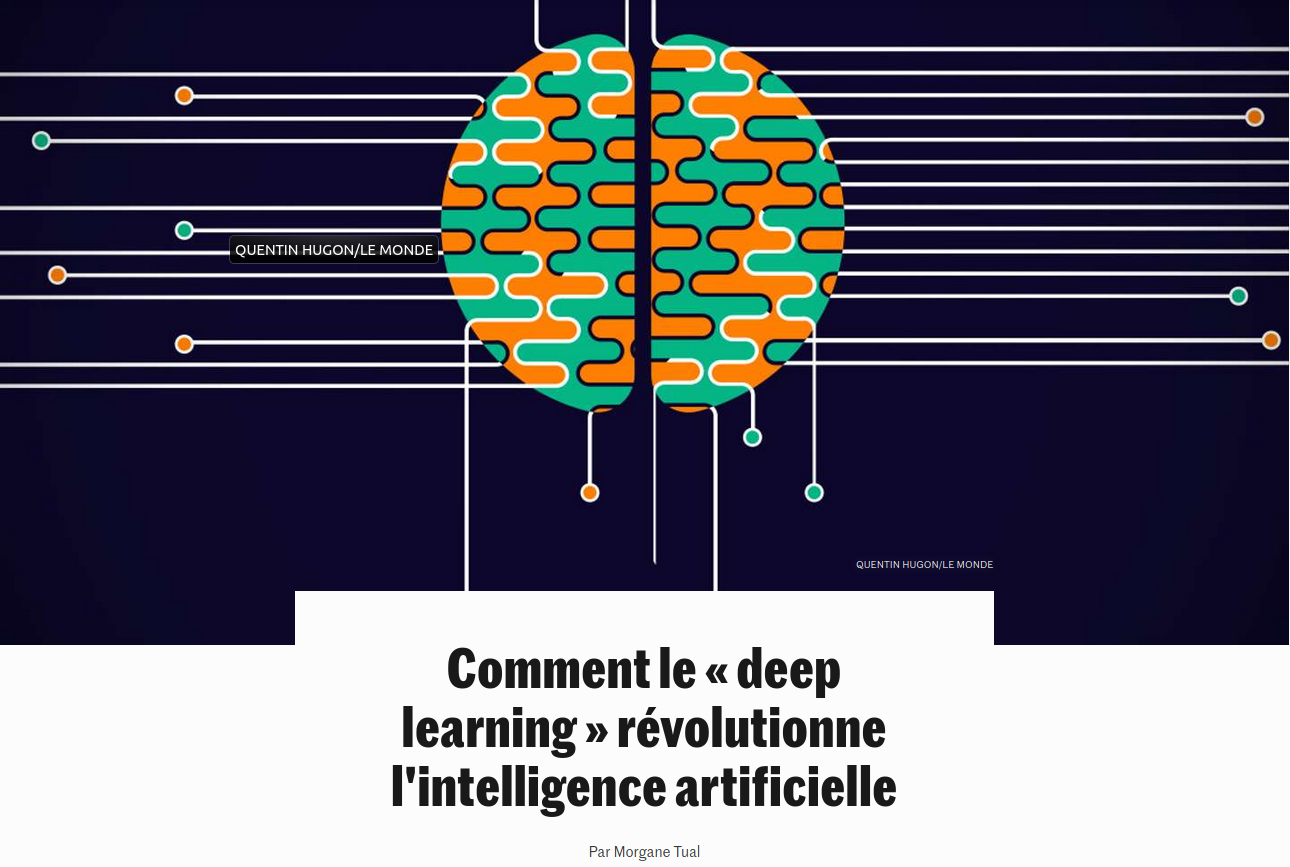
\includegraphics[height=0.5\textheight]{lemonde-juillet2015}
  \caption*{Le Monde, juillet 2015}
\end{figure}


\end{frame}

%%%%%%%%%%%%%%%%%%%%%%%%%%%%%%%%%%%%
\begin{frame}{The rise of deep learning}

\begin{figure}[ht]
  \centering
  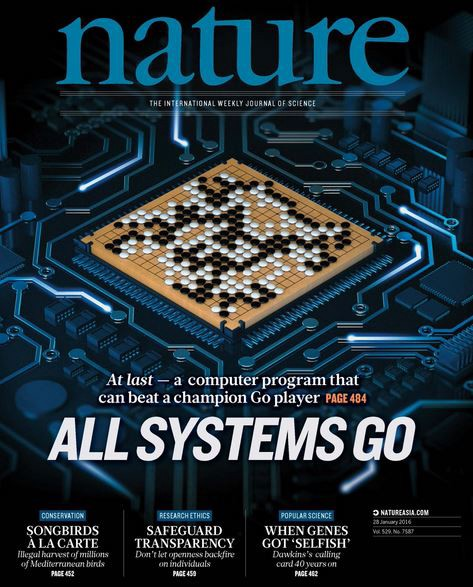
\includegraphics[height=0.5\textheight]{nature_go}
  \caption*{Nature, 2016}
\end{figure}


\end{frame}


%%%%%%%%%%%%%%%%%%%%%%%%%%%%%%%%%%%%
\begin{frame}{The rise of deep learning}

\begin{figure}[ht]
  \centering
  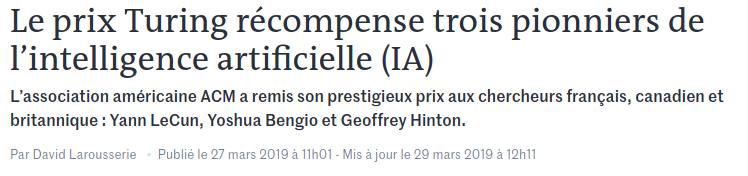
\includegraphics[width=0.7\textwidth]{lemonde27mars2019}
  \caption*{Le Monde, mars 2019}
\end{figure}


\end{frame}

%%%%%%%%%%%%%%%%%%%%%%%%%%%%%%%%%%%%
\begin{frame}{The rise of deep learning}


\begin{figure}[ht]
  \centering
  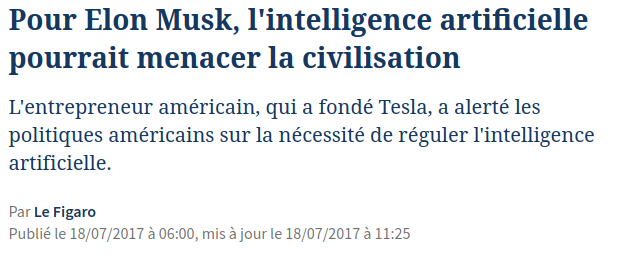
\includegraphics[width=0.7\textwidth]{le_figaro_musk}
  \caption*{Le Figaro, juillet 2017}
\end{figure}



\end{frame}


%%%%%%%%%%%%%%%%%%%%%%%%%%%%%%%%%%%%%%%%%%%%%%%%%%
\section{Differentiable programming}

%%%%%%%%%%%%%%%%%%%%%%%%%%%%%%%%%%%%
\begin{frame}{Differentiable programming}

\begin{block}{Definition}
  Differentiable programming is an algorithmic framework where differentiable operators are combined together to build complex systems. The parameters of the system can then be optimized via gradient descent thanks to \alert{back-propagation}.
\end{block}

\begin{itemize}
\item In our case, \alert{computational graphs} will be used to compute a \alert{loss} function $\loss$, which depends on the input of the system $\X$ and its parameters $\param = \{\param_1, \ldots, \param_q\}$.

\end{itemize}

\end{frame}
%%%%%%%%%%%%%%%%%%%%%%%%%%%%%%%%%%%%
\begin{frame}{Gradient descent in the scalar case}

\begin{columns}
  \begin{column}{.5\textwidth}
    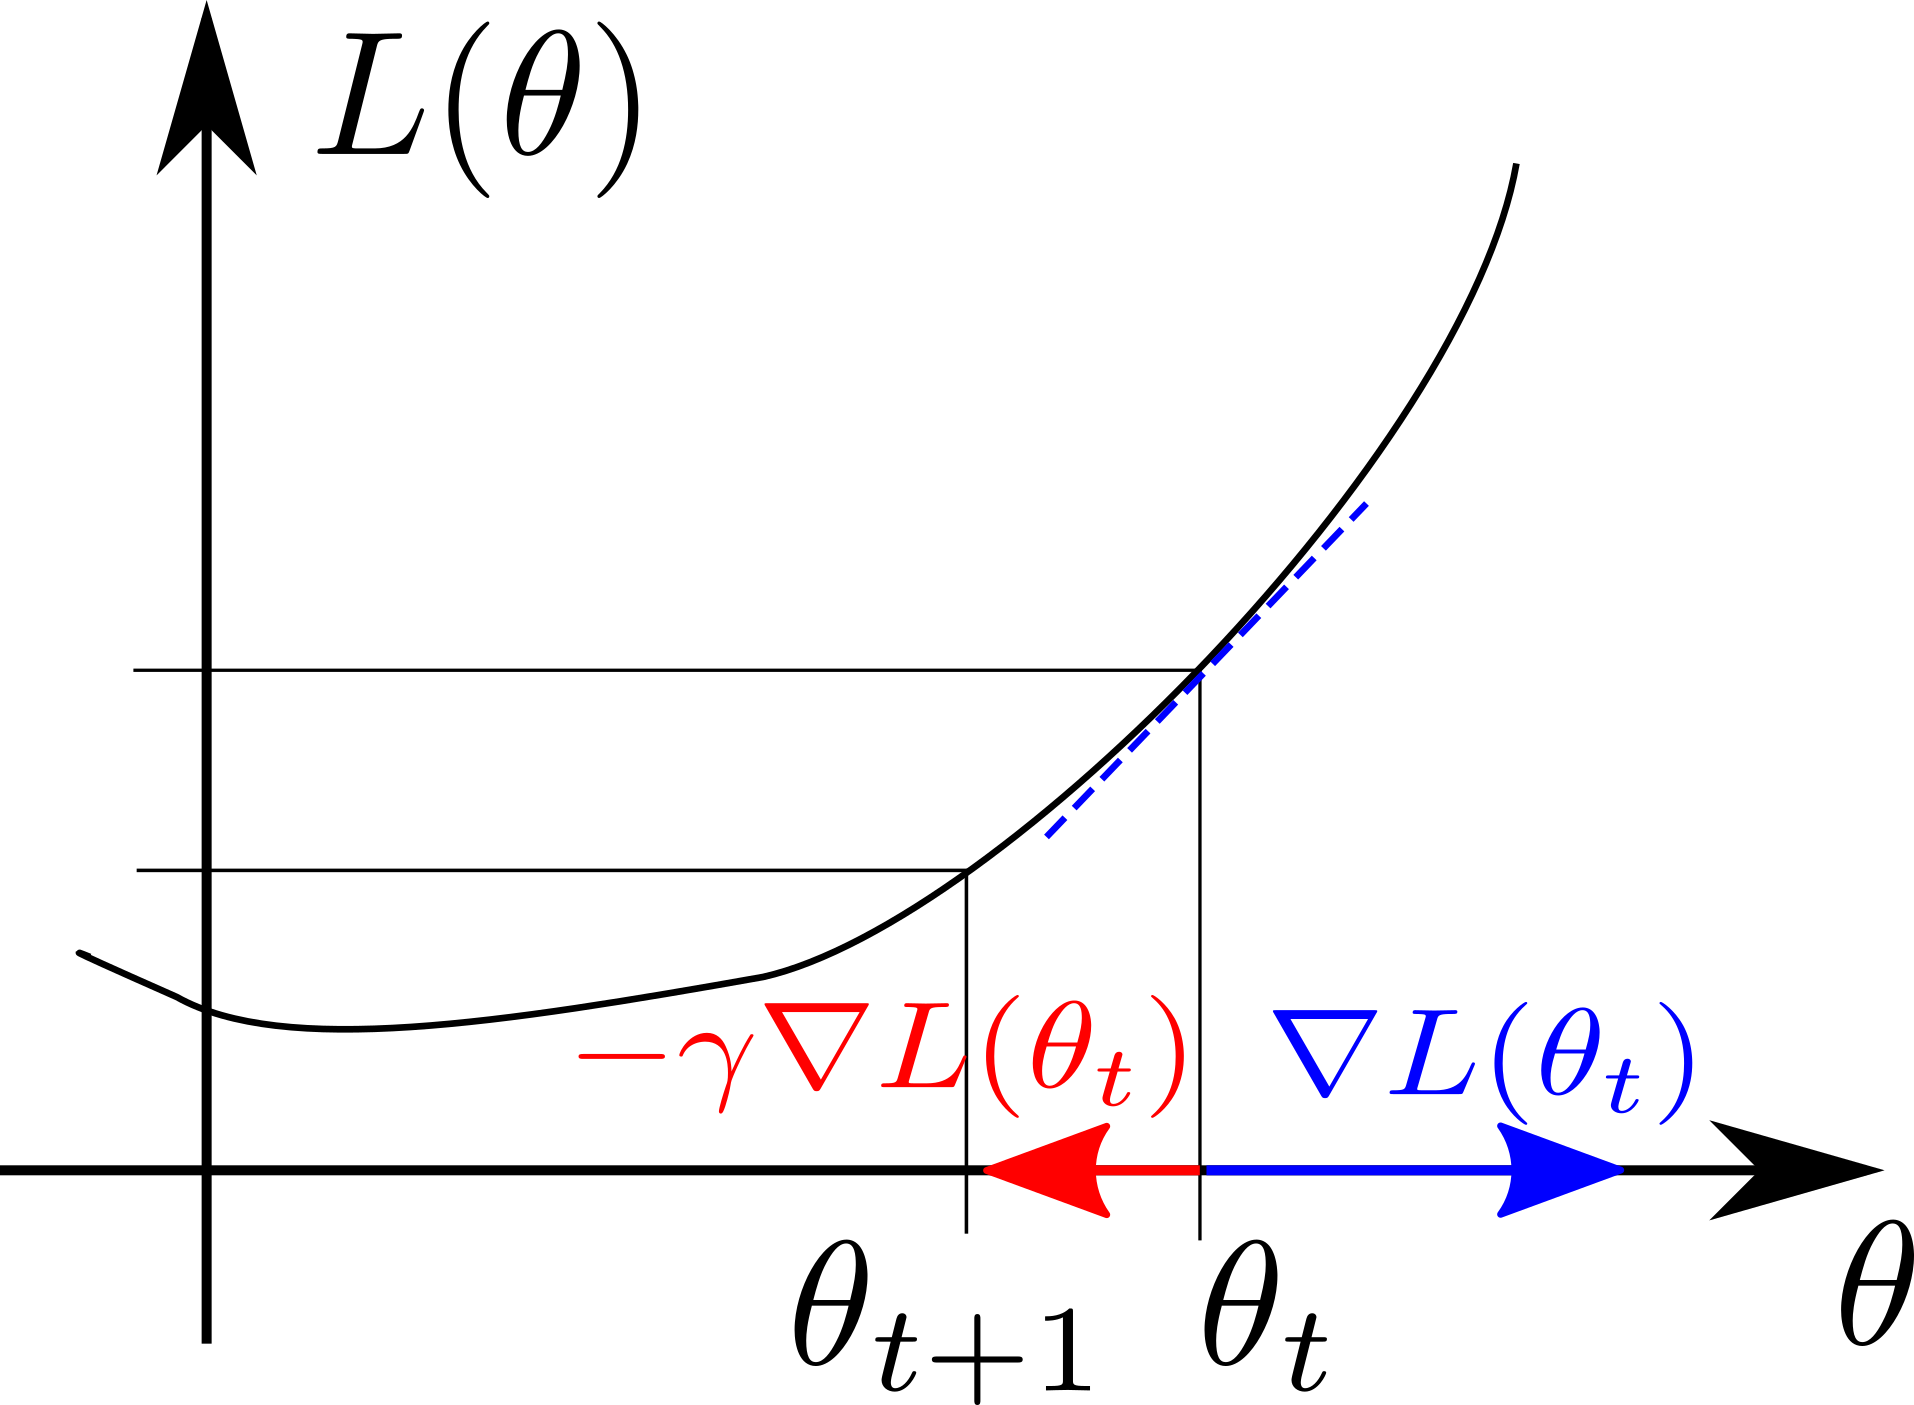
\includegraphics[width=\textwidth]{gradient_descent}
  \end{column}

  \begin{column}{.5\textwidth}
    \[
    \param_{t+1} = \param_t - \lr\nabla \loss(\param_t)
    \]
  \end{column}
\end{columns}

\end{frame}



%%%%%%%%%%%%%%%%%%%%%%%%%%%%%%%%%%%%
\begin{frame}{How to minimize a function?}

  \begin{columns}
    \begin{column}{.6\textwidth}
      \begin{figure}
        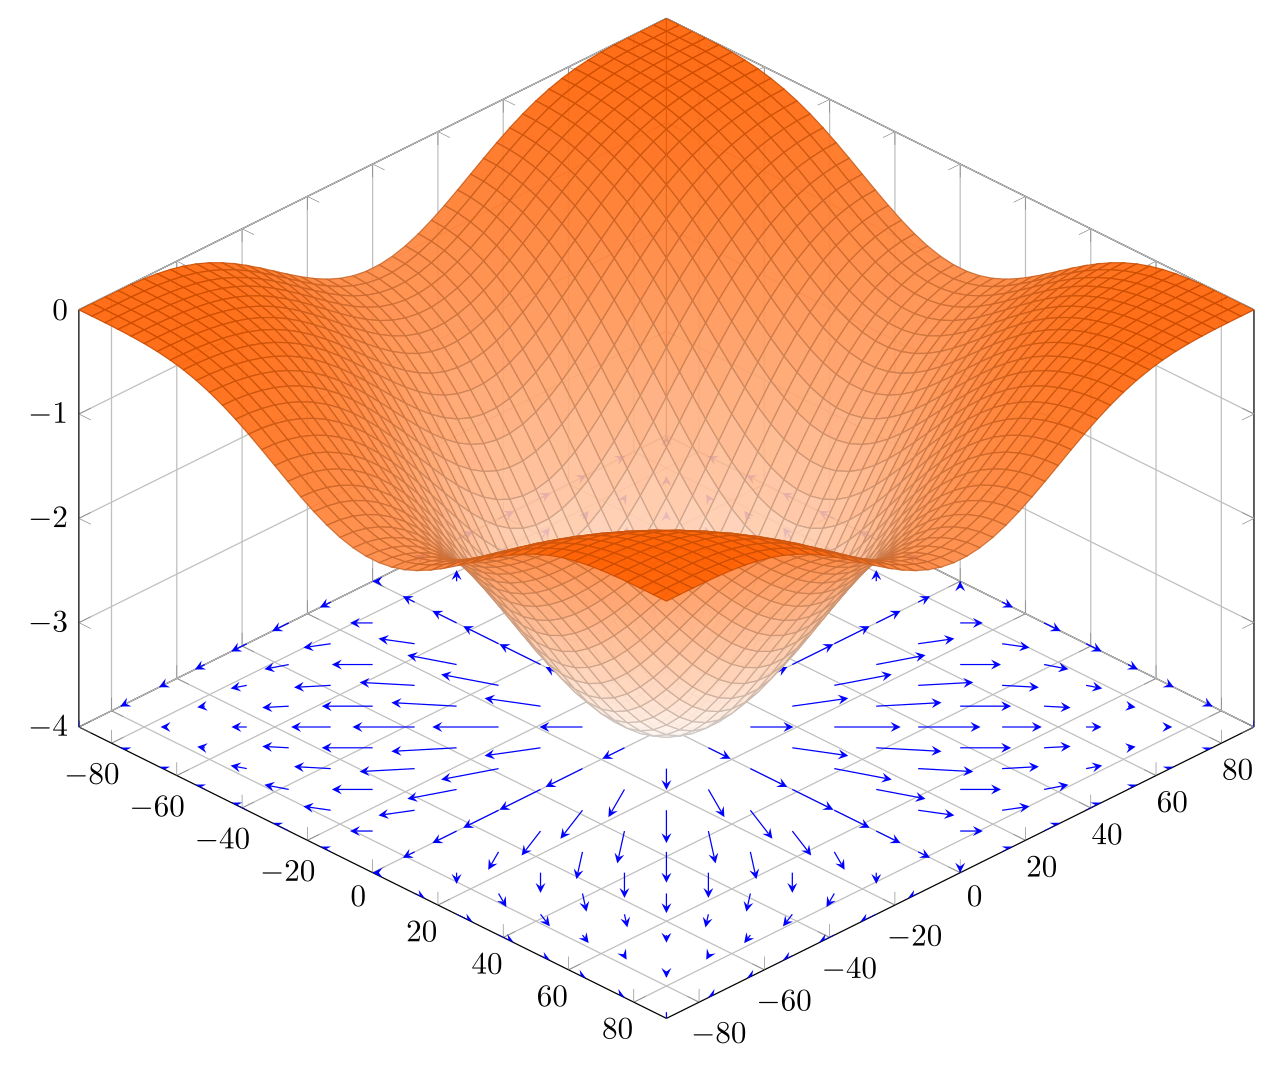
\includegraphics[height=5cm]{3d-gradient-cos.png}
        \source{By MartinThoma, CC0, https://commons.wikimedia.org/}
      \end{figure}
    \end{column}


    \begin{column}{.4\textwidth}
      \begin{block}{Definition: gradient}
        Let $\loss $ be a derivable function from $\R^n$ into $\R$. Its gradient $\nabla\loss$ is:
        \[
        \nabla \loss (\param) =
        \begin{pmatrix}
          \frac{\partial \loss}{\partial \param_1}(\param)\\
          \vdots \\
          \frac{\partial \loss}{\partial \param_n}(\param)
        \end{pmatrix}
        \]

      \end{block}
    \end{column}
  \end{columns}


\end{frame}

%%%%%%%%%%%%%%%%%%%%%%%%%%%%%%%%%%%%
\begin{frame}{Computational graph}

\begin{block}{Definition}
  A computational graph is a direct acyclic graph such that:
  \begin{itemize}
  \item A node is a mathematical operator
  \item To each edge is associated a value (scalar, vector, matrix, tensor, $\ldots$)
  \item Each node can compute the values of its output edges from the values of its input edges
  \end{itemize}
\end{block}

Computing a \emph{forward pass} through the graph means choosing its input values, and then progressively computing the values of all edges.


\end{frame}


%%%%%%%%%%%%%%%%%%%%%%%%%%%%%%%%%%%%
\begin{frame}{Computational graph example}
  Computational graph of:
  \[
  \sigma(w_1x + w_2y + b)
  \]
  where $\sigma$ is the sigmoid function: $\sigma(x) = \frac{1}{1 + e^{-x}}$

\vspace{3em}
\pause

  \centering
  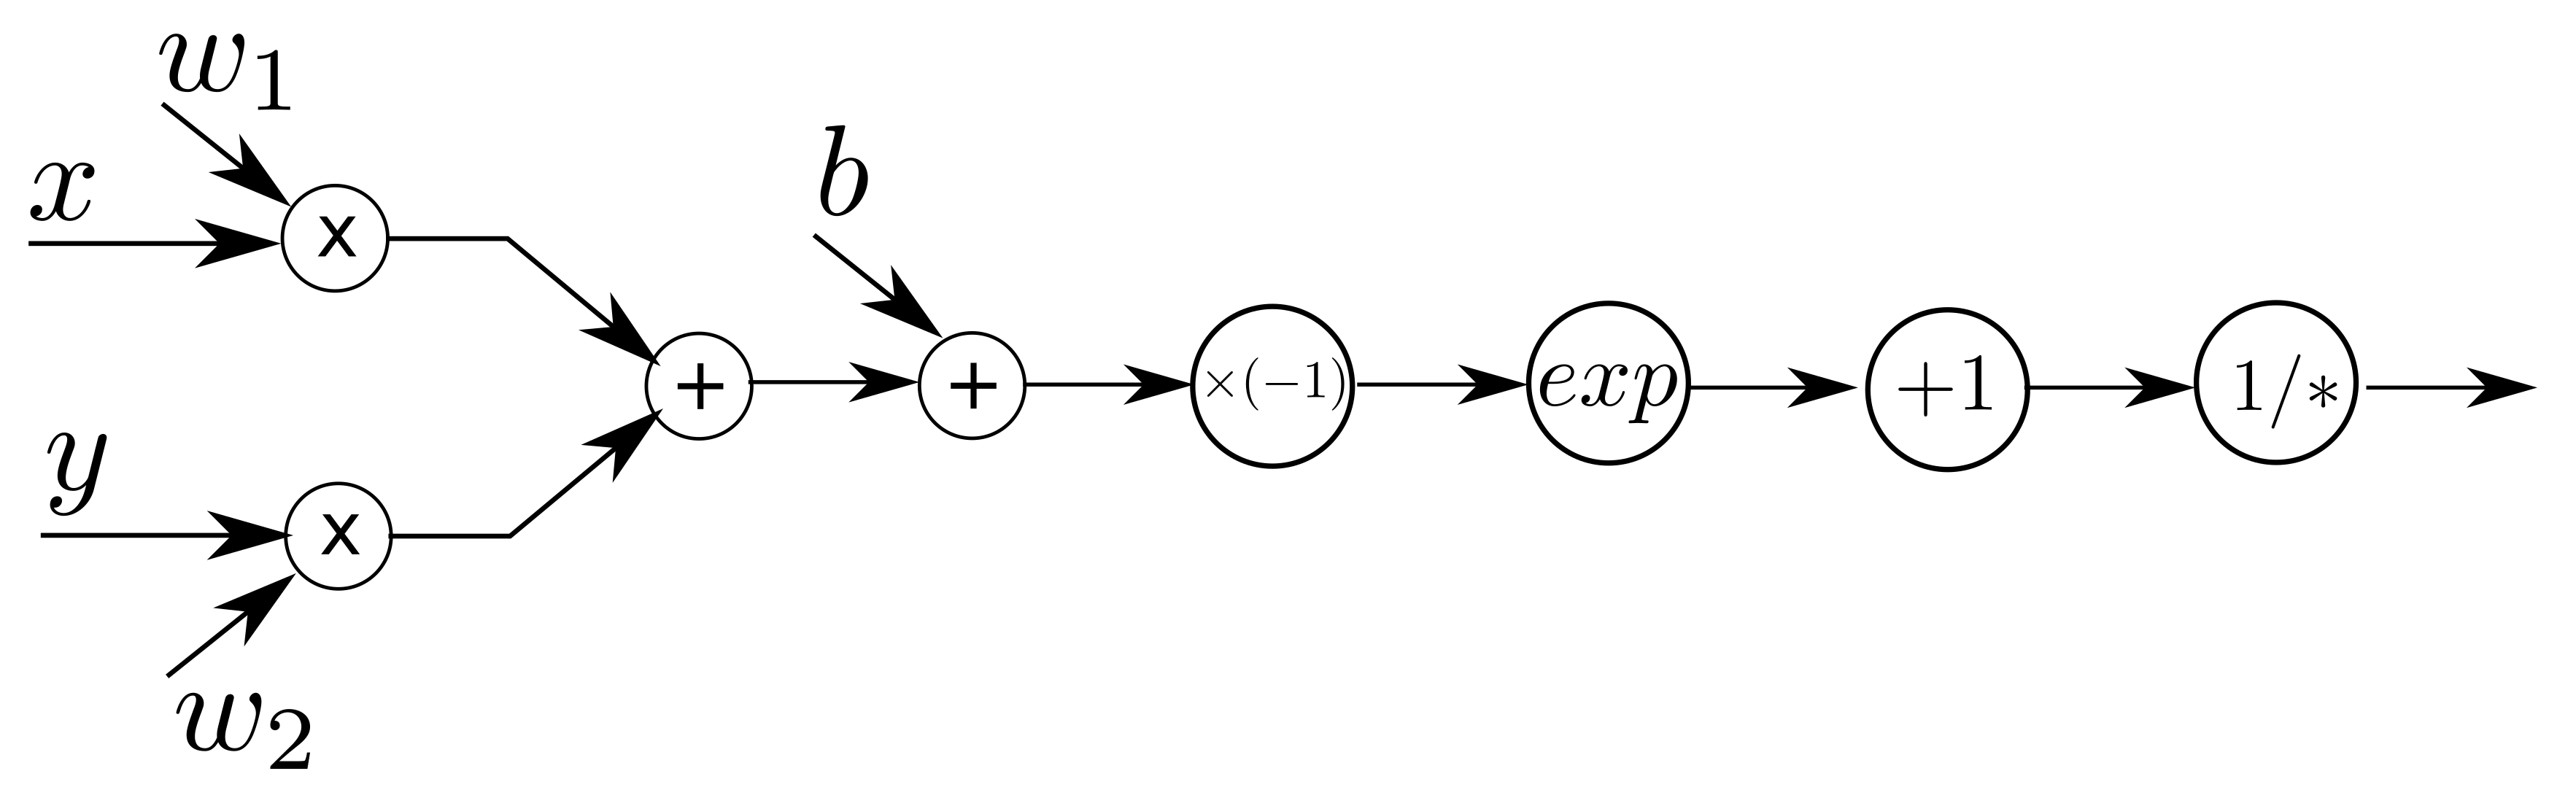
\includegraphics[width=0.7\textwidth]{comp_graph2}\\
  \pause
  The graph can be represented at different levels of detail:
  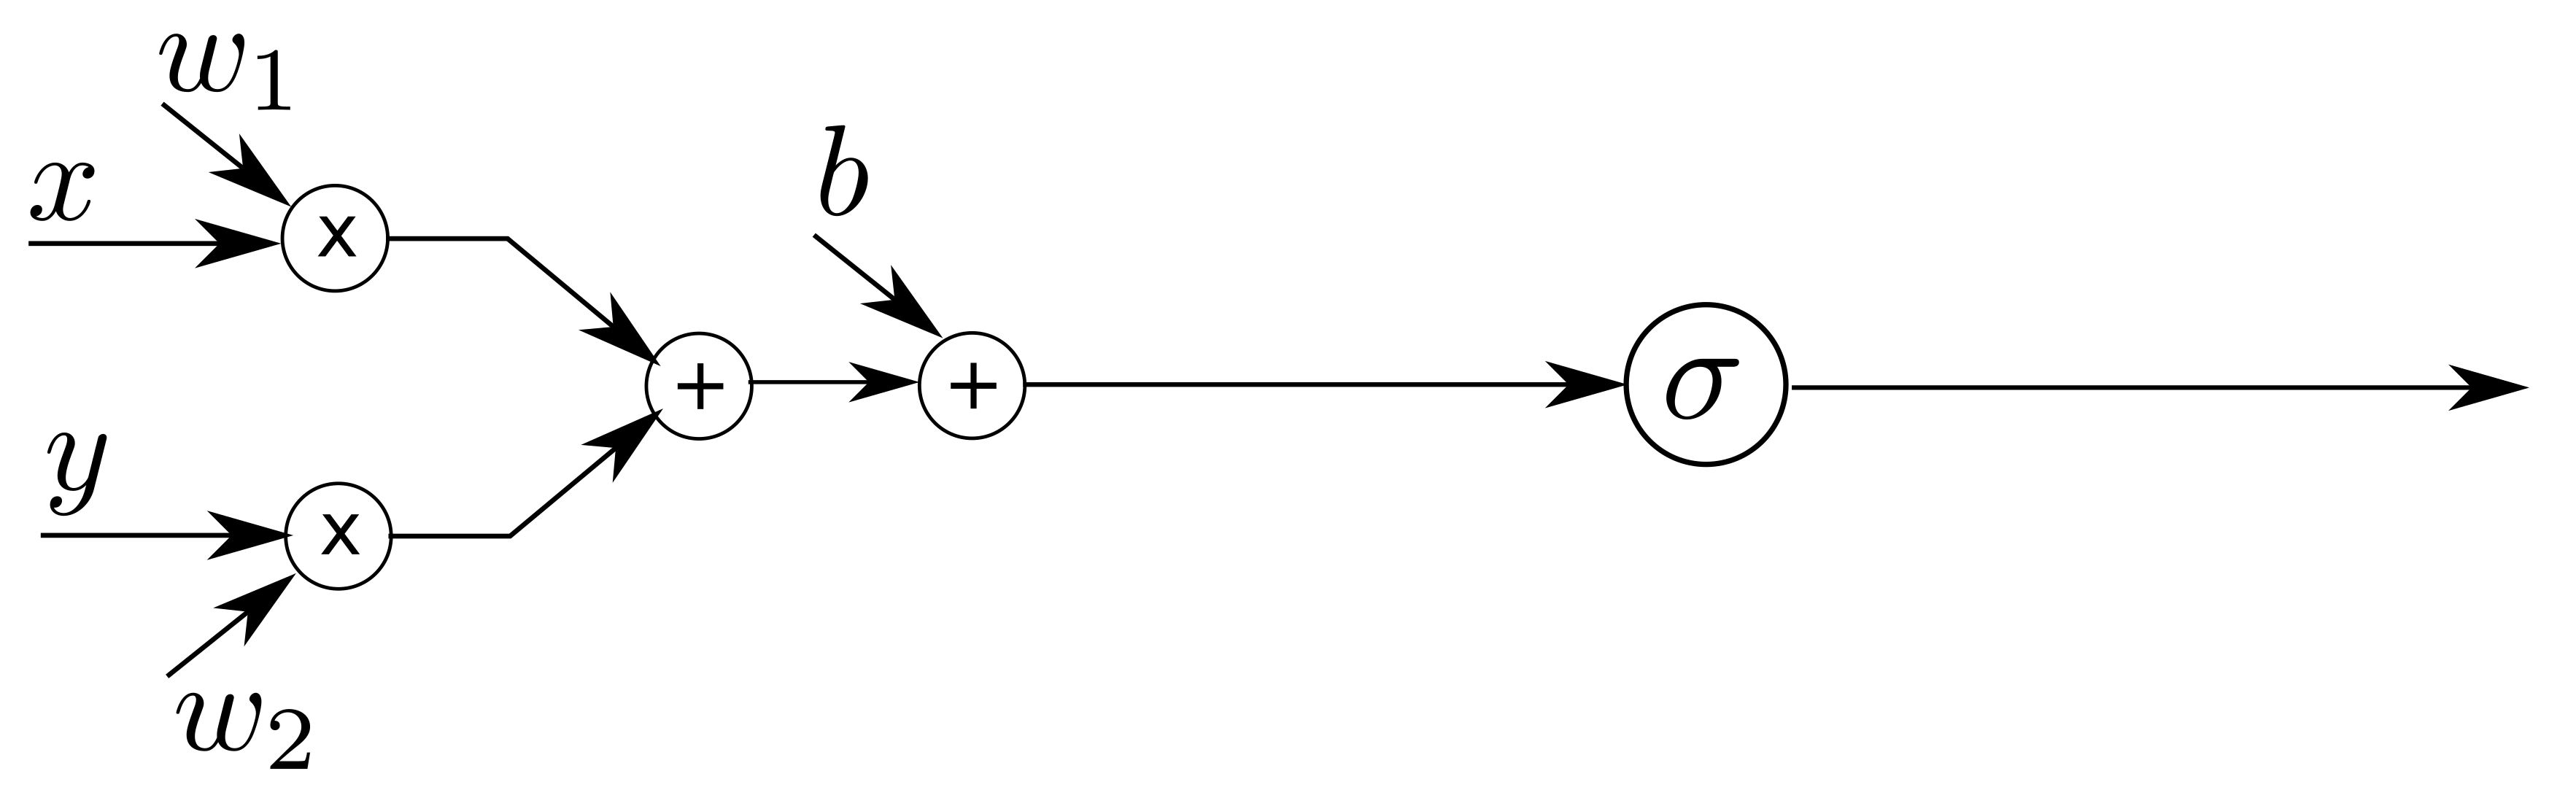
\includegraphics[width=0.7\textwidth]{comp_graph}

\end{frame}

%%%%%%%%%%%%%%%%%%%%%%%%%%%%%%%%%%%%
\begin{frame}{Gradient descent applied to computational graphs}

  In the case of computational graphs, the loss $\loss$ depends on each parameter $\param_i$ via the composition of several simple functions. In order to compute the gradient $\nabla_{\param}\loss$ we will make extensive use of the chain rule theorem.

  \begin{block}{Chain rule theorem}
    Let $f_1$ and $f_2$ be two derivable real functions ($\R \rightarrow \R$). Then for all $x$ in $\R$:   :
    \[
     (f_2 \circ f_1)'(x) = f_2'(f_1(x)).f_1'(x)
    \]
  \end{block}


\begin{block}{Leibniz notation}
  Let us introduce variables $x$, $y$ and $z$:
  \[x \xrightarrow{f_1} y \xrightarrow{f_2} z\]

  Then:
  \[\dv{z}{x} = \dv{z}{y} \cdot \dv{y}{x} \]

\end{block}

\end{frame}


%%%%%%%%%%%%%%%%%%%%%%%%%%%%%%%%%%%%
\begin{frame}{The backpropagation algorithm}

  \begin{itemize}
  \item The backpropagation algorithm is used in a computational graph to efficiently compute the partial derivatives of the loss with respect to each parameter of the network.
  \item One can trace the origins of the method to the sixties
  \item It was first applied to NN in the eighties \cite{werbos_applications_1982, lecun_procedure_1985}
  \end{itemize}


\end{frame}


%%%%%%%%%%%%%%%%%%%%%%%%%%%%%%%%%%%%
\begin{frame}{The backpropagation algorithm: intuition}

  \begin{itemize}
  \item Given a computational graph, the main idea is to compute the local partial derivatives during a forward pass
    \item Then, during a backward pass, the partial derivatives of the loss with respect to each parameter is computed
  \end{itemize}


\end{frame}





%%%%%%%%%%%%%%%%%%%%%%%%%%%%%%%%%%%%
\begin{frame}<handout>{Simple backpropagation example}

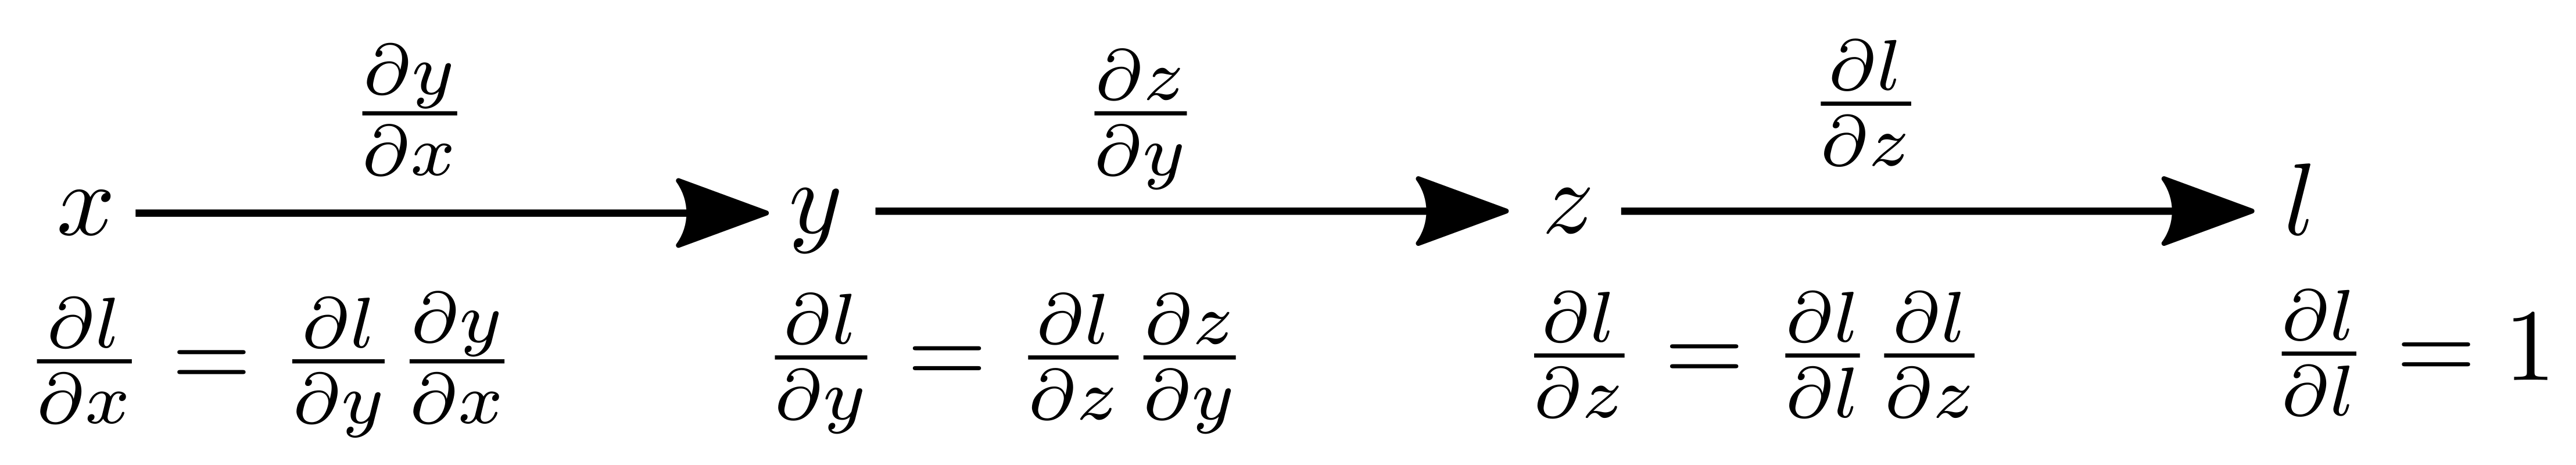
\includegraphics[width=\textwidth]{bp_simple.png}

\end{frame}

%%%%%%%%%%%%%%%%%%%%%%%%%%%%%%%%%%%%
\begin{frame}<beamer>{Simple backpropagation example}

\only<1>{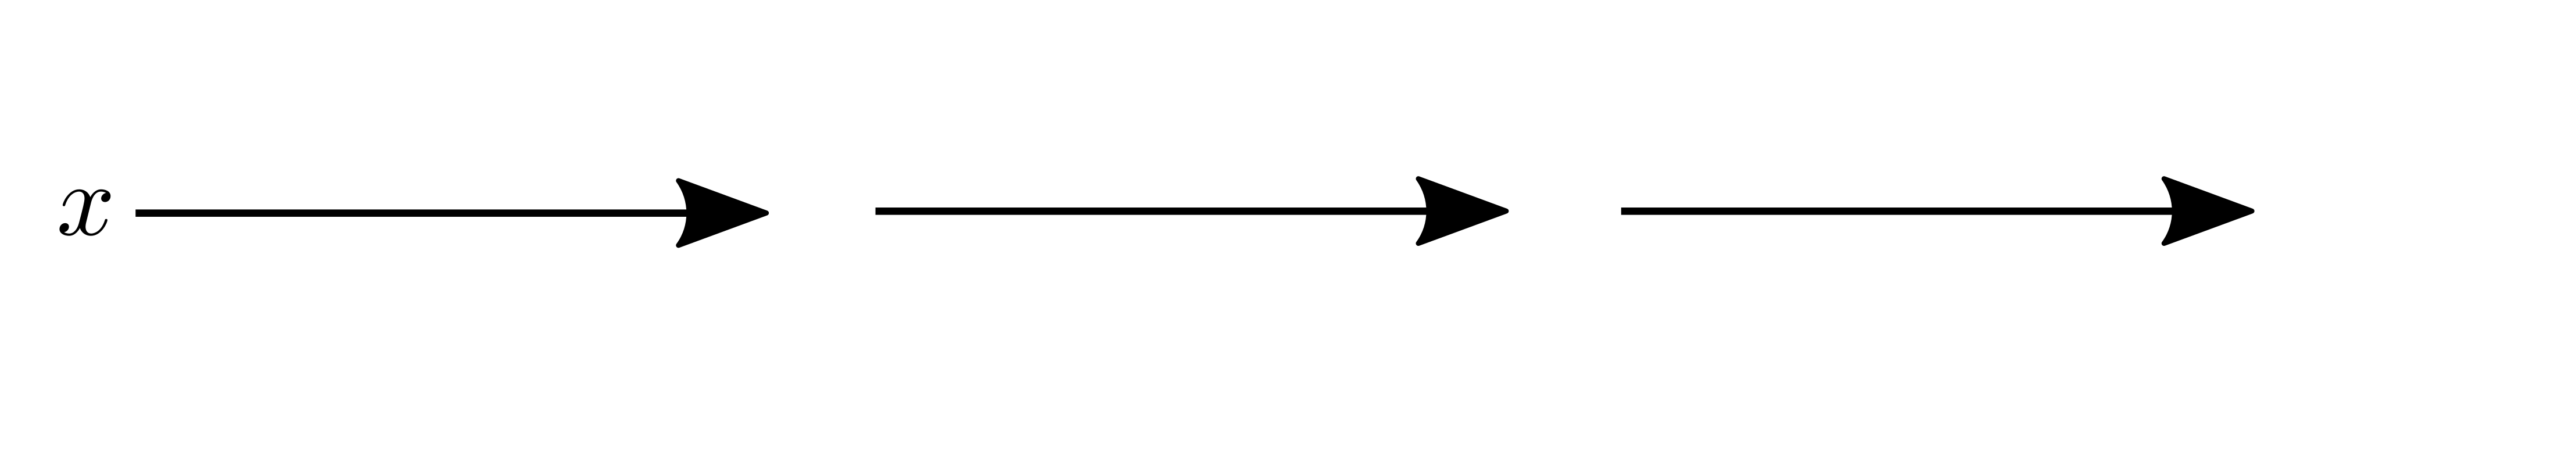
\includegraphics[width=\textwidth]{bp_simple_1.png}}
\only<2>{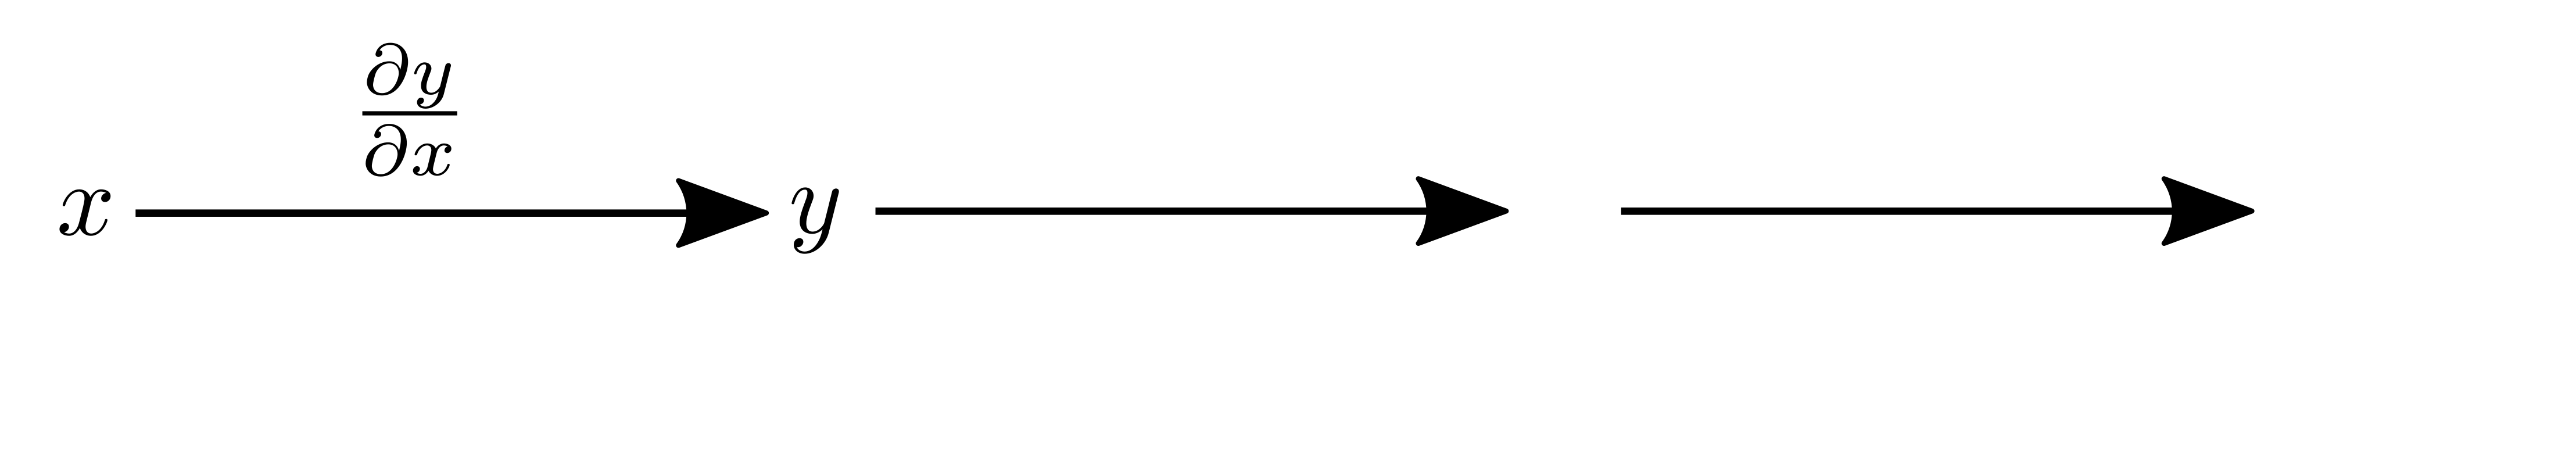
\includegraphics[width=\textwidth]{bp_simple_2.png}}
\only<3>{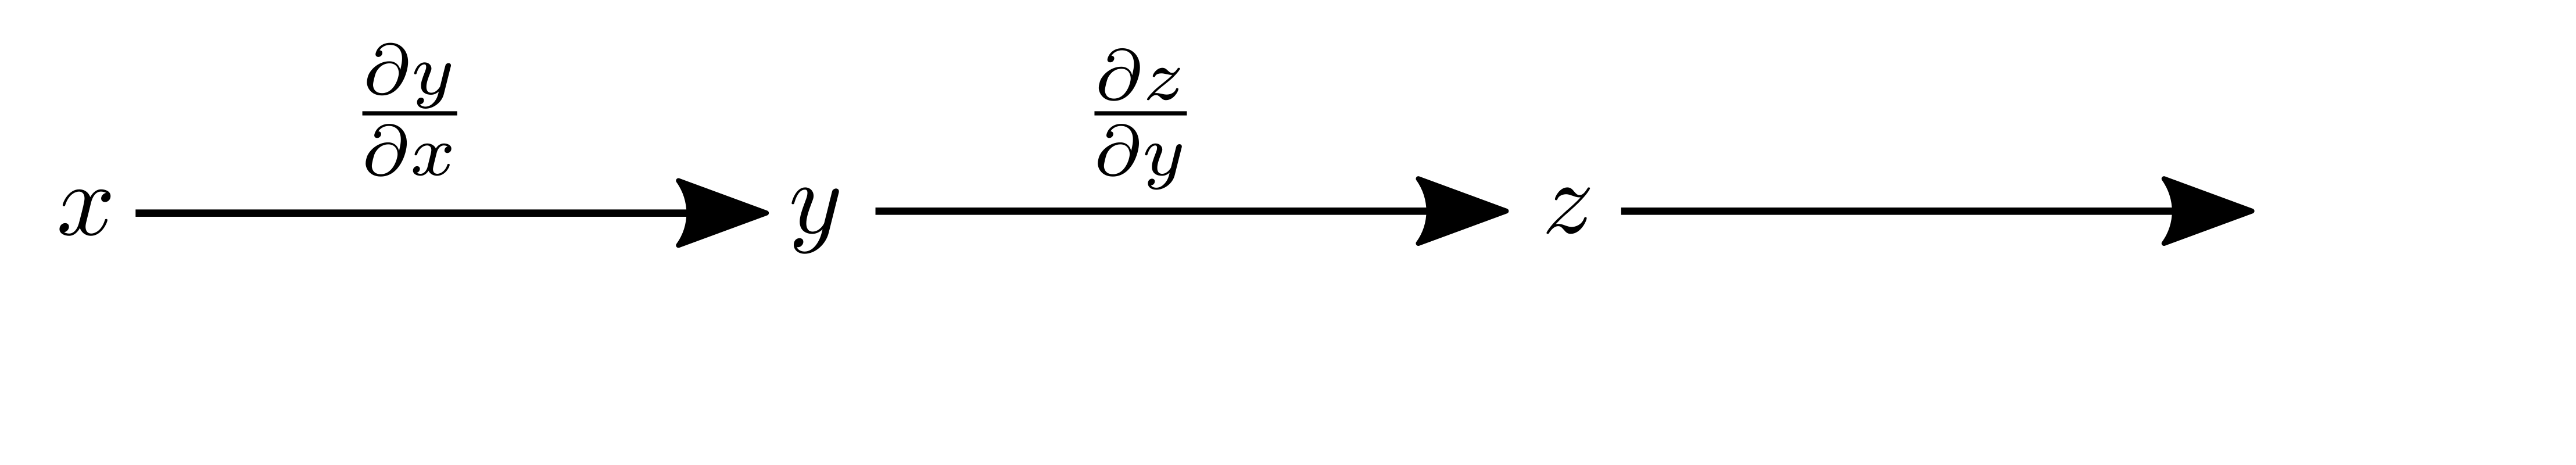
\includegraphics[width=\textwidth]{bp_simple_3.png}}
\only<4>{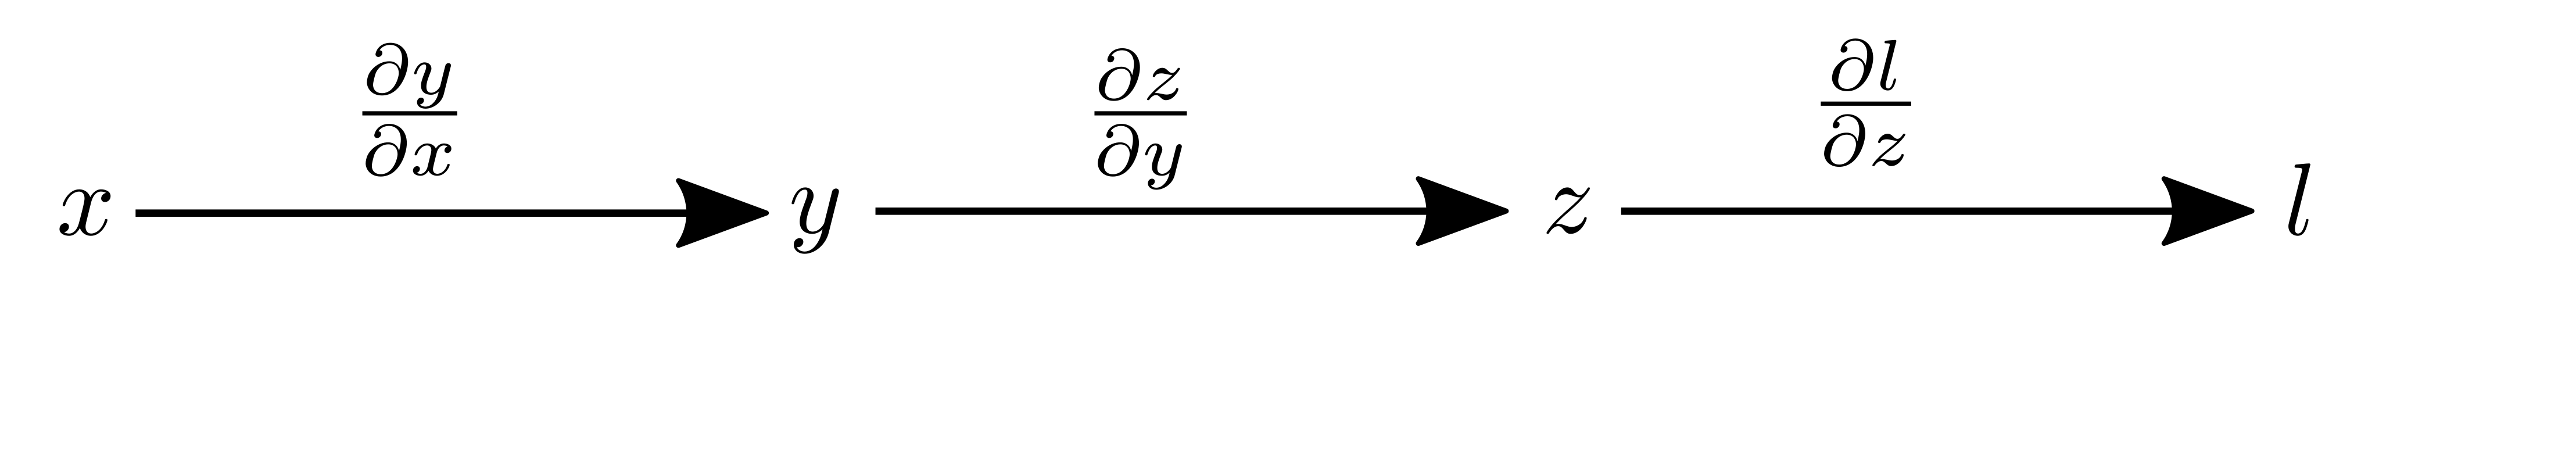
\includegraphics[width=\textwidth]{bp_simple_4.png}}
\only<5>{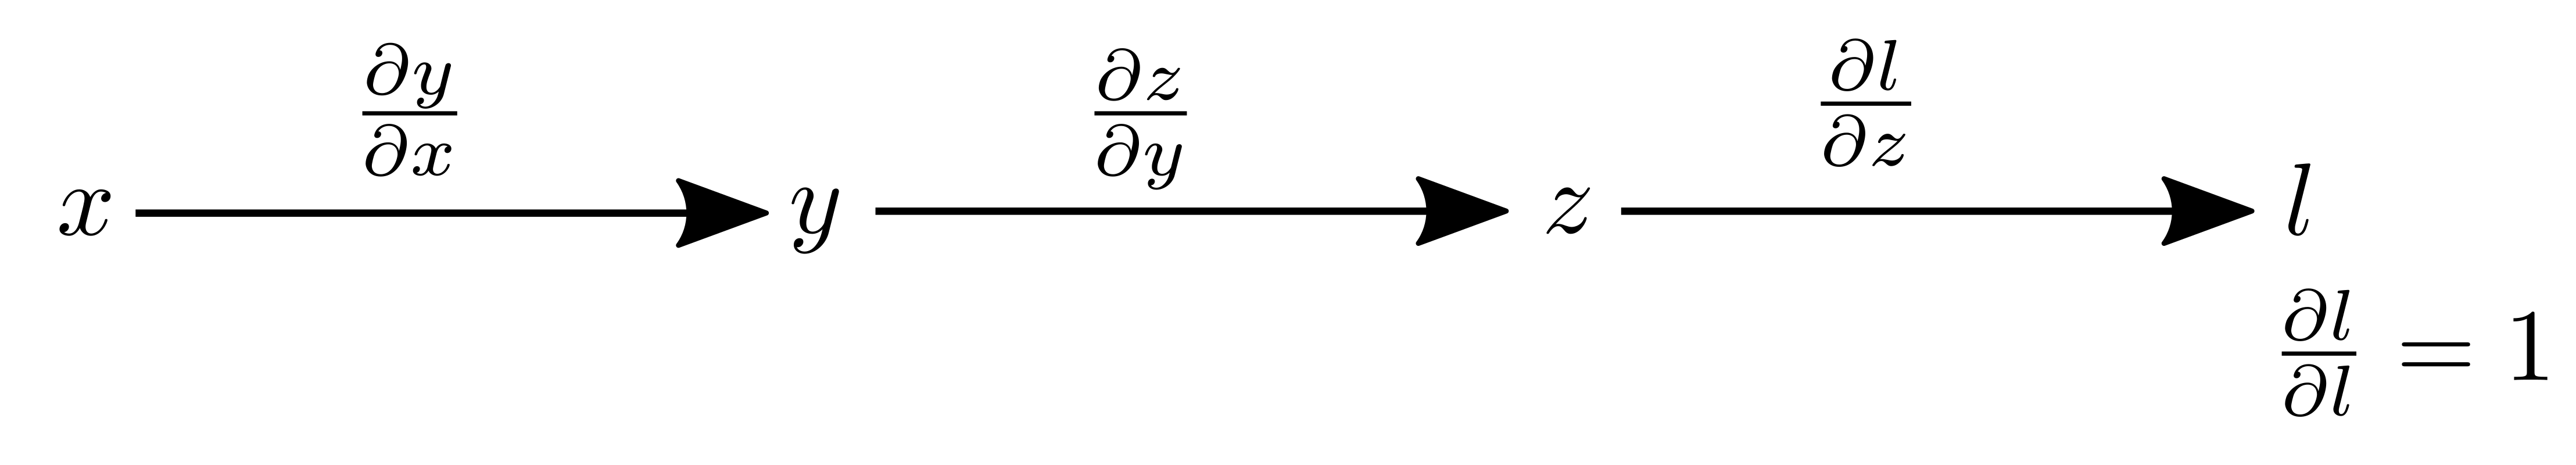
\includegraphics[width=\textwidth]{bp_simple_5.png}}
\only<6>{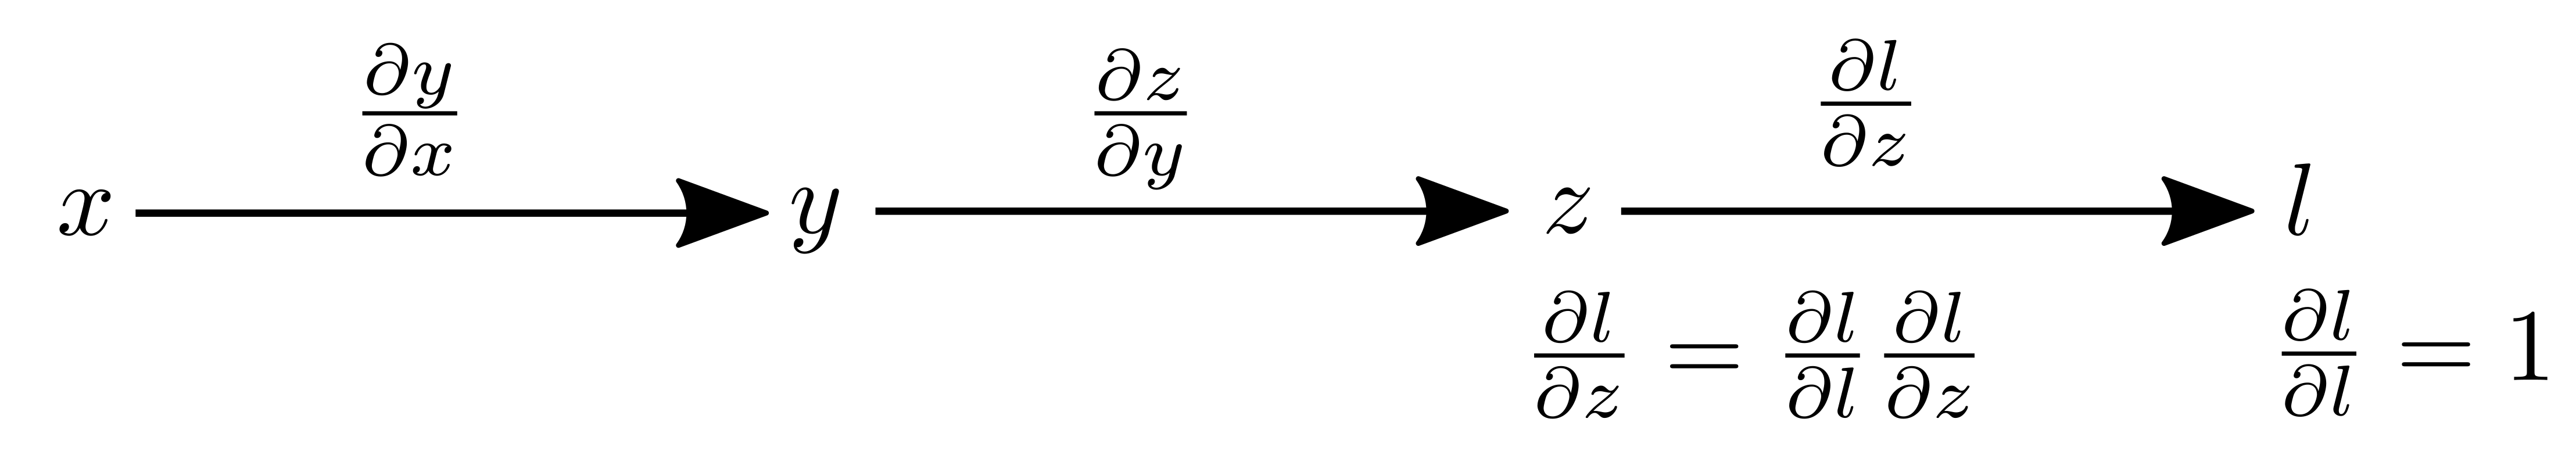
\includegraphics[width=\textwidth]{bp_simple_6.png}}
\only<7>{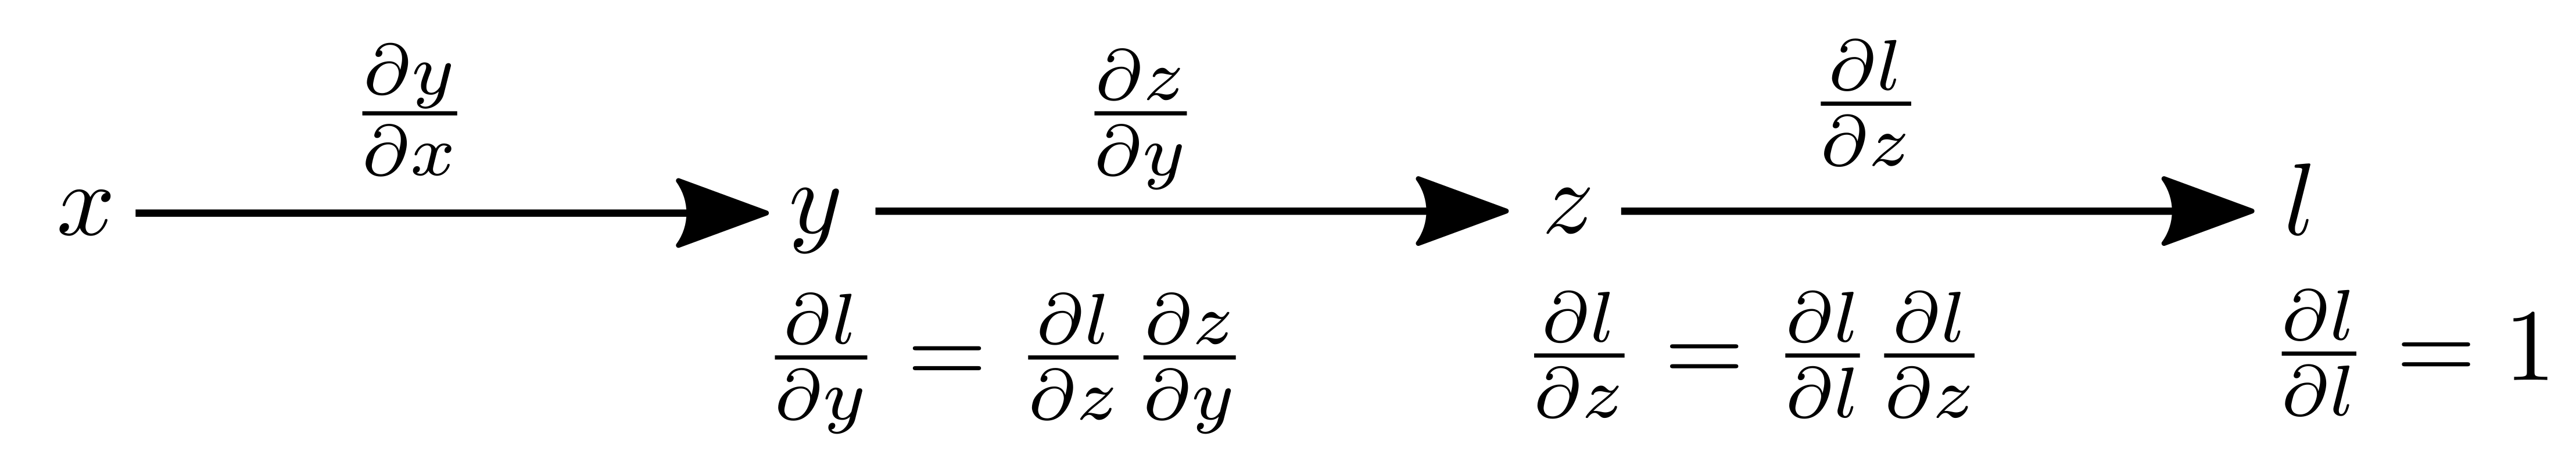
\includegraphics[width=\textwidth]{bp_simple_7.png}}
\only<8>{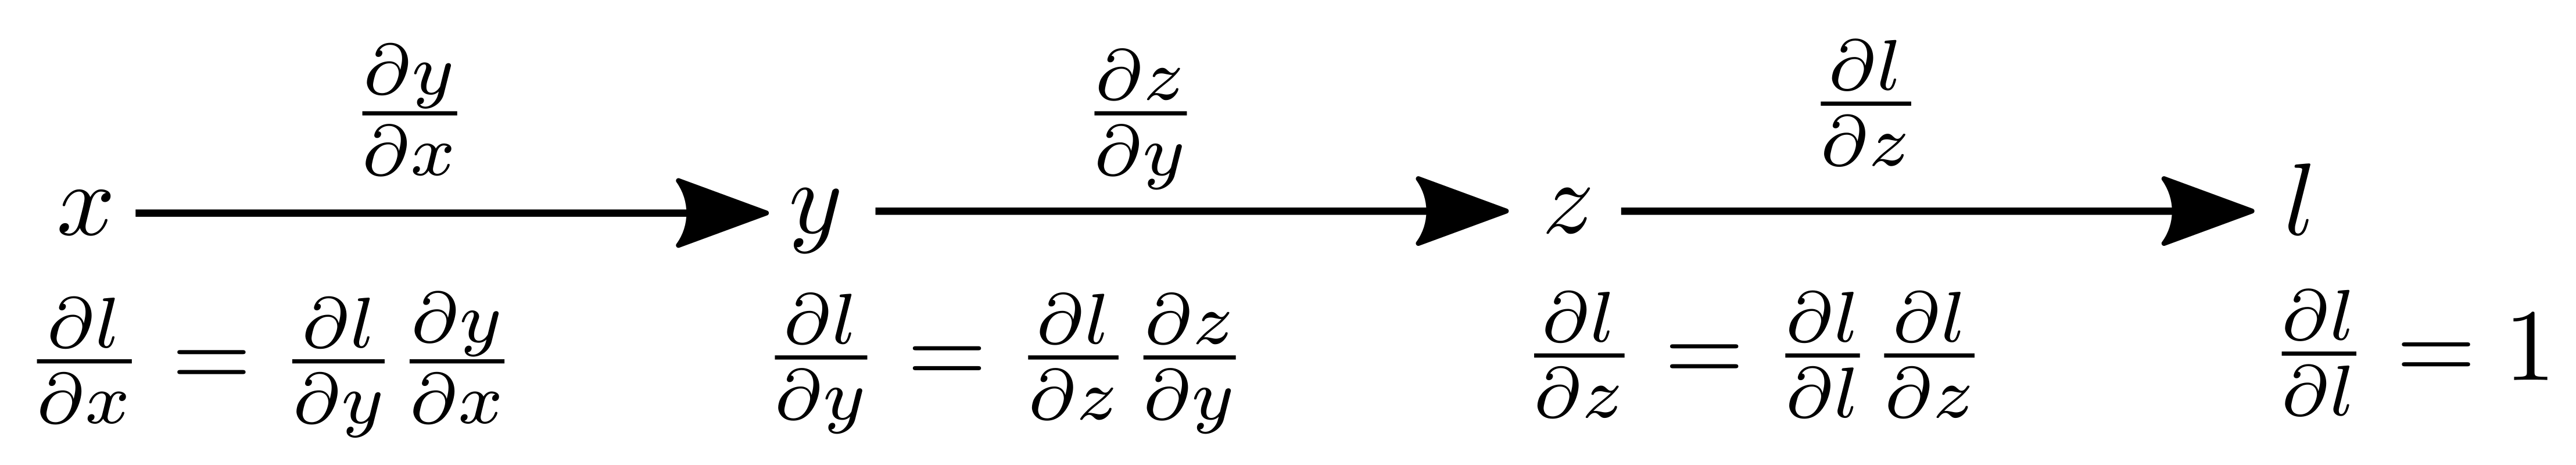
\includegraphics[width=\textwidth]{bp_simple_8.png}}

\end{frame}

%%%%%%%%%%%%%%%%%%%%%%%%%%%%%%%%%%%%%%%%%%%%%%%%%%
\frame{
\frametitle{Feed-forward neural networks}

\begin{block}{Definition}
  \begin{itemize}
  \item A feed-forward neural networks is a computational graph without cycles
  \item Its computing units, the neurons, are organized in \alert{layers}
  \end{itemize}

\end{block}

\begin{figure}
  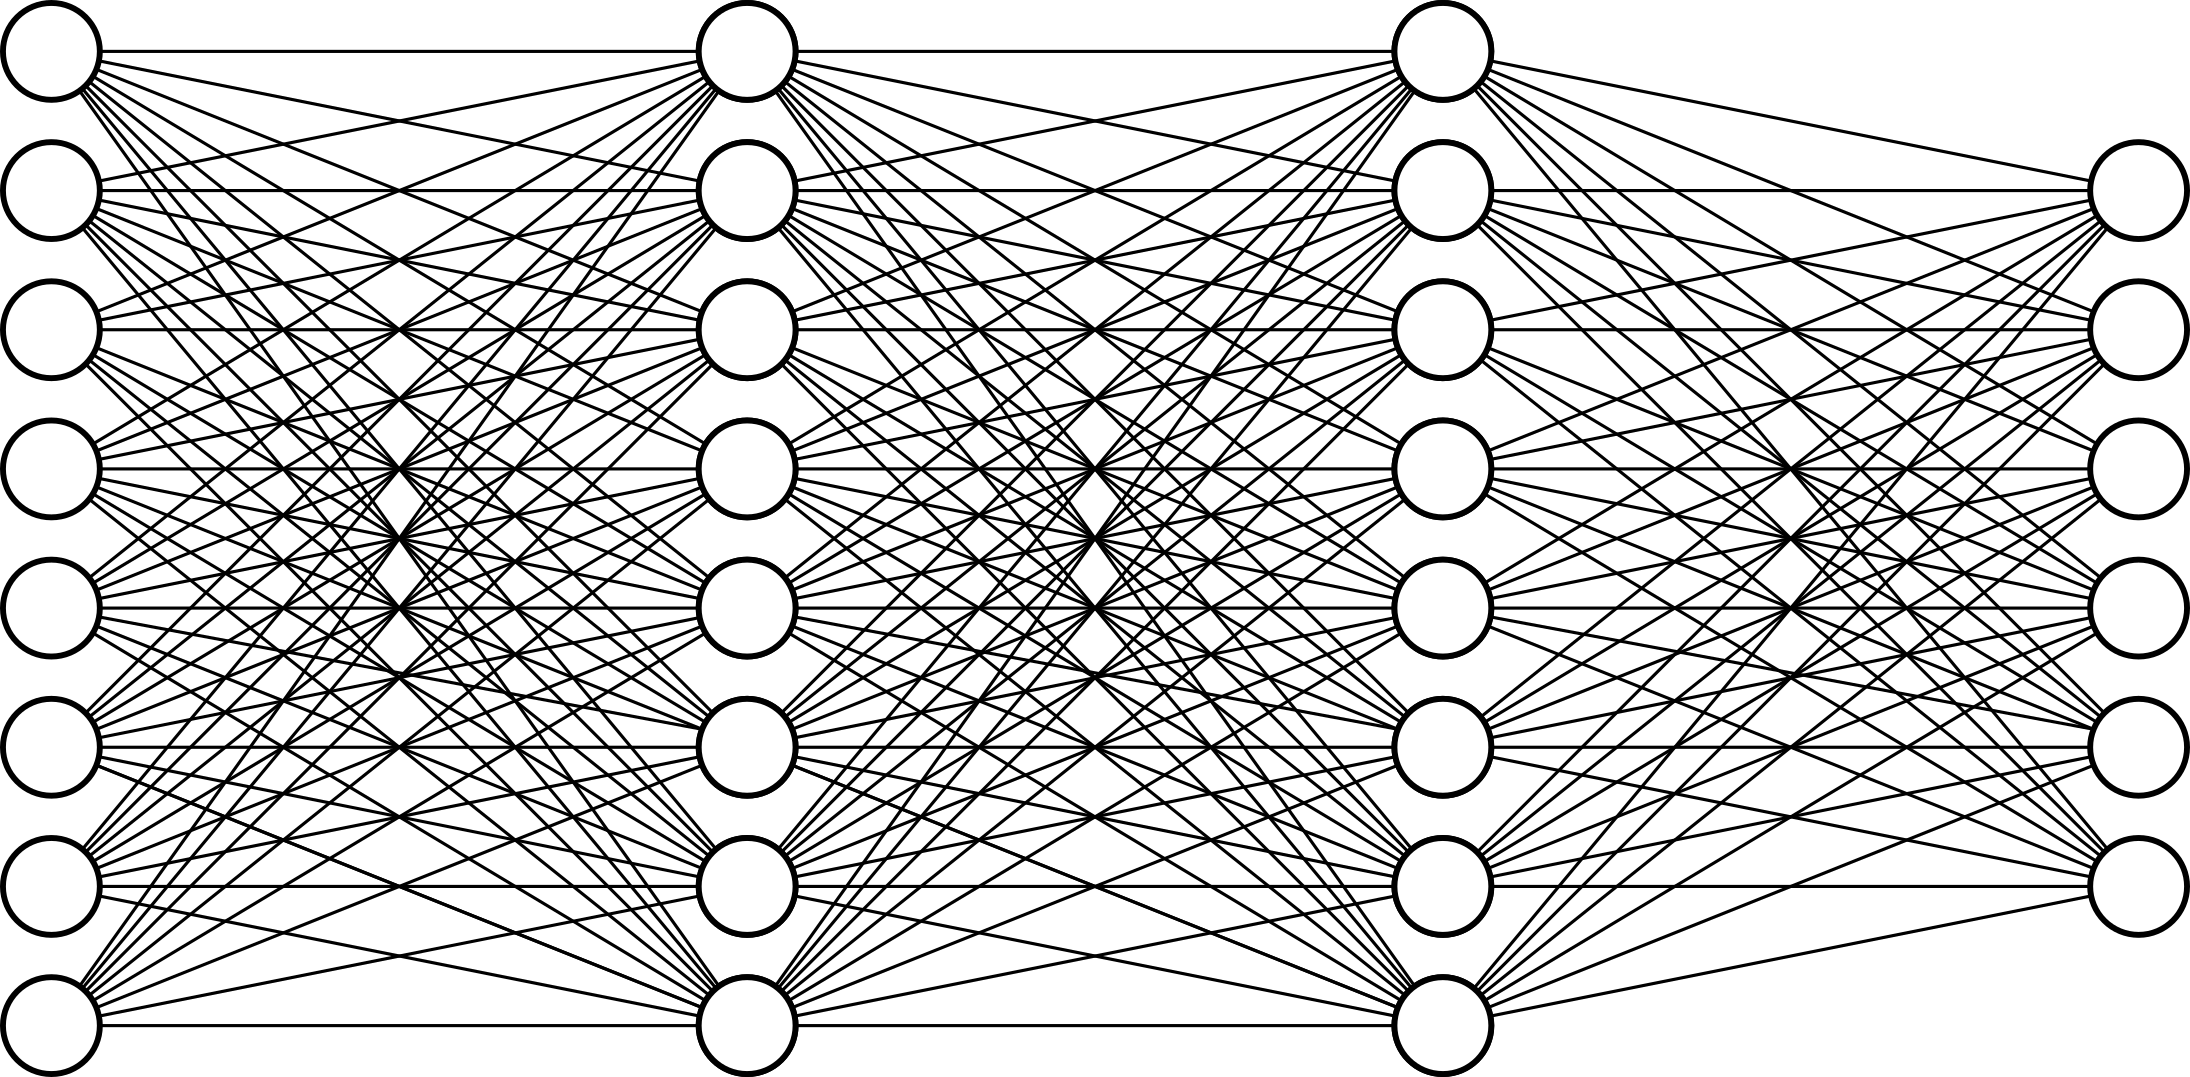
\includegraphics[height=3cm]{mini_reseau3_bis.png}
\end{figure}


}


%%%%%%%%%%%%%%%%%%%%%%%%%%%%%%%%%%%%
\begin{frame}{Artificial neuron}

    \begin{figure}
      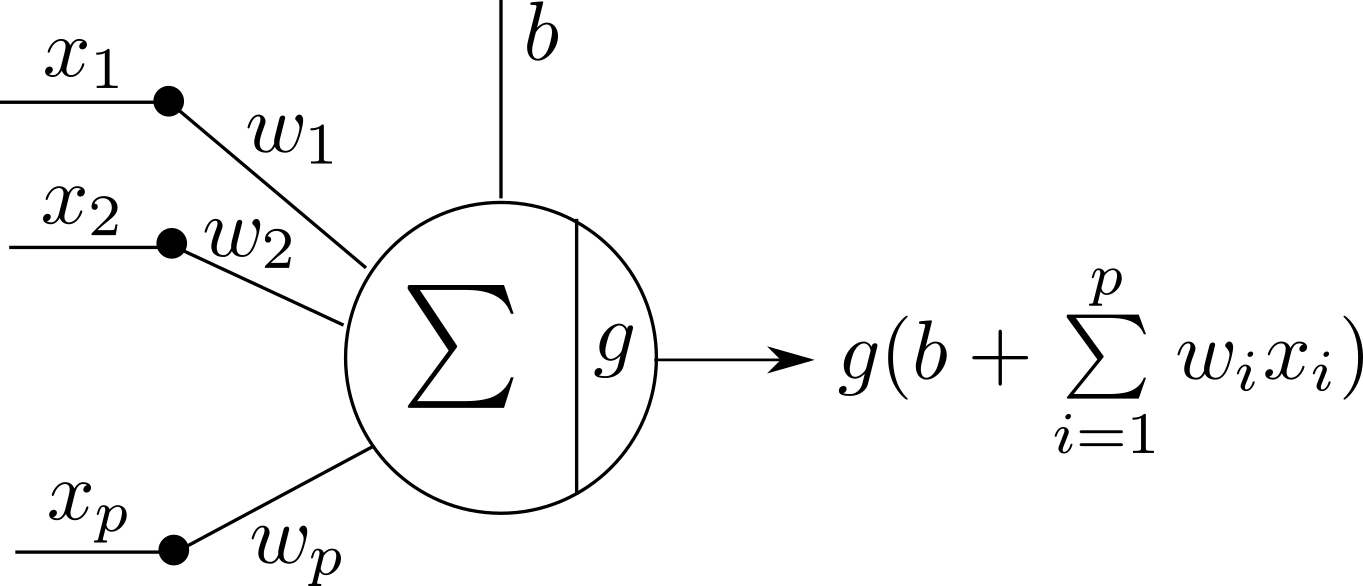
\includegraphics[height=3cm]{neurone_representation_compacte}
    \end{figure}

\end{frame}

%%%%%%%%%%%%%%%%%%%%%%%%%%%%%%%%%%%%%%%%%%%%%%
\frame{
\frametitle{Notations}

\begin{columns}

  \begin{column}{.5\textwidth}
\begin{figure}
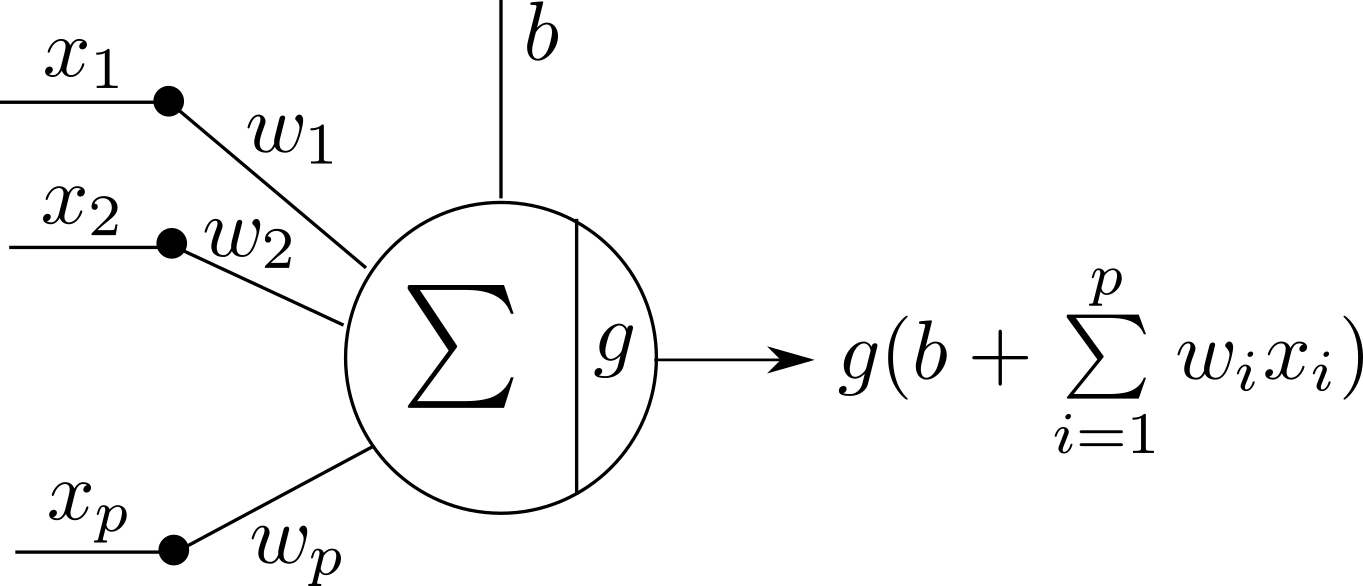
\includegraphics[height=2cm]{neurone_representation_compacte}
\end{figure}
\end{column}

  \begin{column}{.5\textwidth}
  With
  \[
  \mathbf{w} =
  \begin{pmatrix}
    w_1 \\
    \vdots \\
    w_p
  \end{pmatrix}
  = (w_1, \ldots, w_p)^T
  \]
  and
  \[
  \x =
  \begin{pmatrix}
    x_1 \\
    \vdots \\
    x_p
  \end{pmatrix}
  = (x_1, \ldots, x_p)^T
  \]
\end{column}

\end{columns}

We can simply write:
\[
\act(b+ \sum\limits_{i=1}^p w_ix_i) = \act(b + \mathbf{w}^T\x)
\]

}


%%%%%%%%%%%%%%%%%%%%%%%%%%%%%%%%%%%%%%%%%%%%%%%%%%
\frame{
\frametitle{Fully-connected layer}

\begin{itemize}
\item A layer is said to be fully-connected (FC) if each of its neurons is connected to all the neurons of the previous layer
  \item  If a FC layer contains $r$ neurons, and the previous layer $q$, then its weights are a 2D dimensional array (a matrix) of size $q \times r$
\end{itemize}

\begin{figure}
  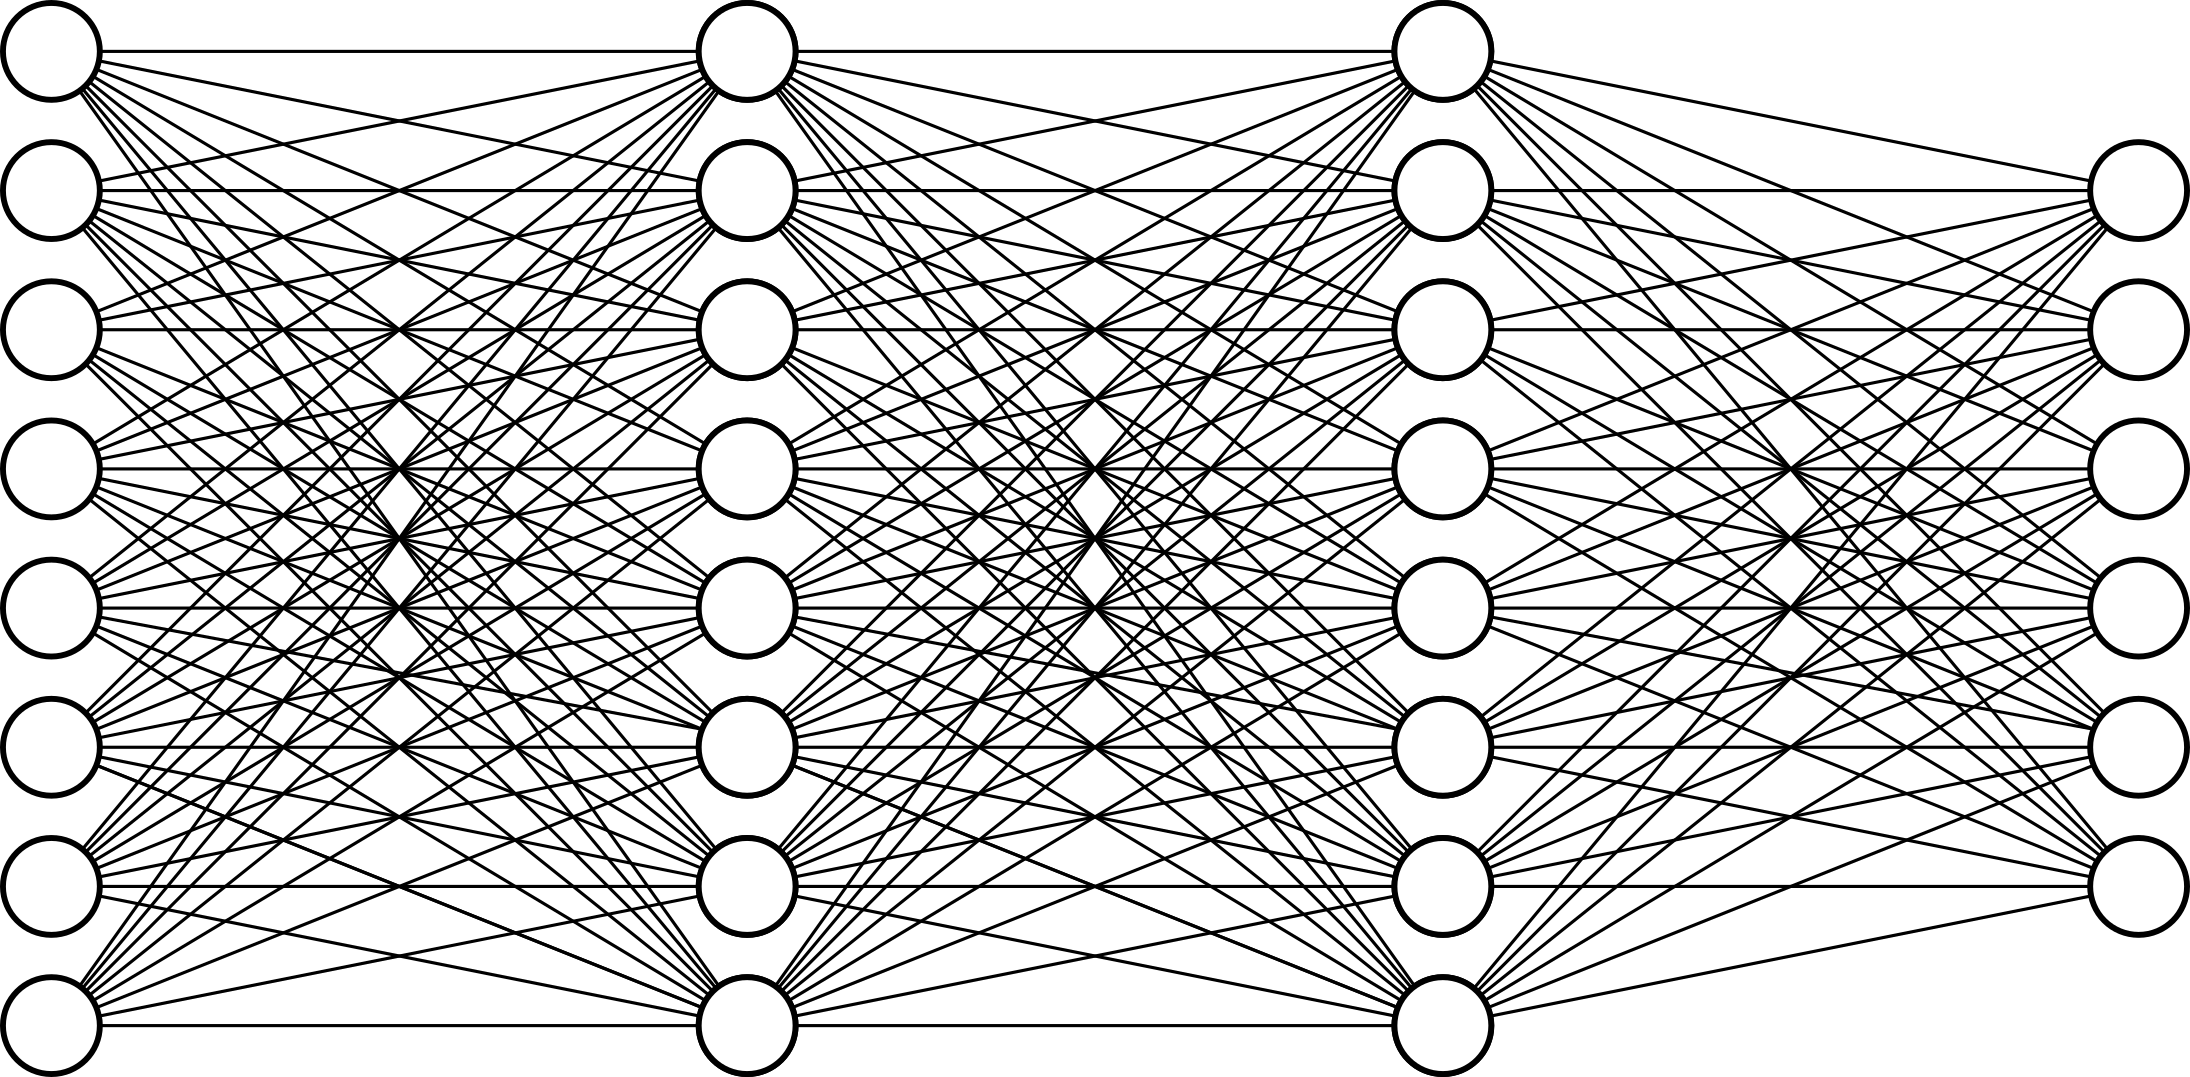
\includegraphics[height=3cm]{mini_reseau3_bis.png}
\end{figure}

}


%%%%%%%%%%%%%%%%%%%%%%%%%%%%%%%%%%%%
\begin{frame}{Graphical representation of NNs}

\begin{columns}
  \begin{column}{.5\textwidth}
    \begin{figure}
      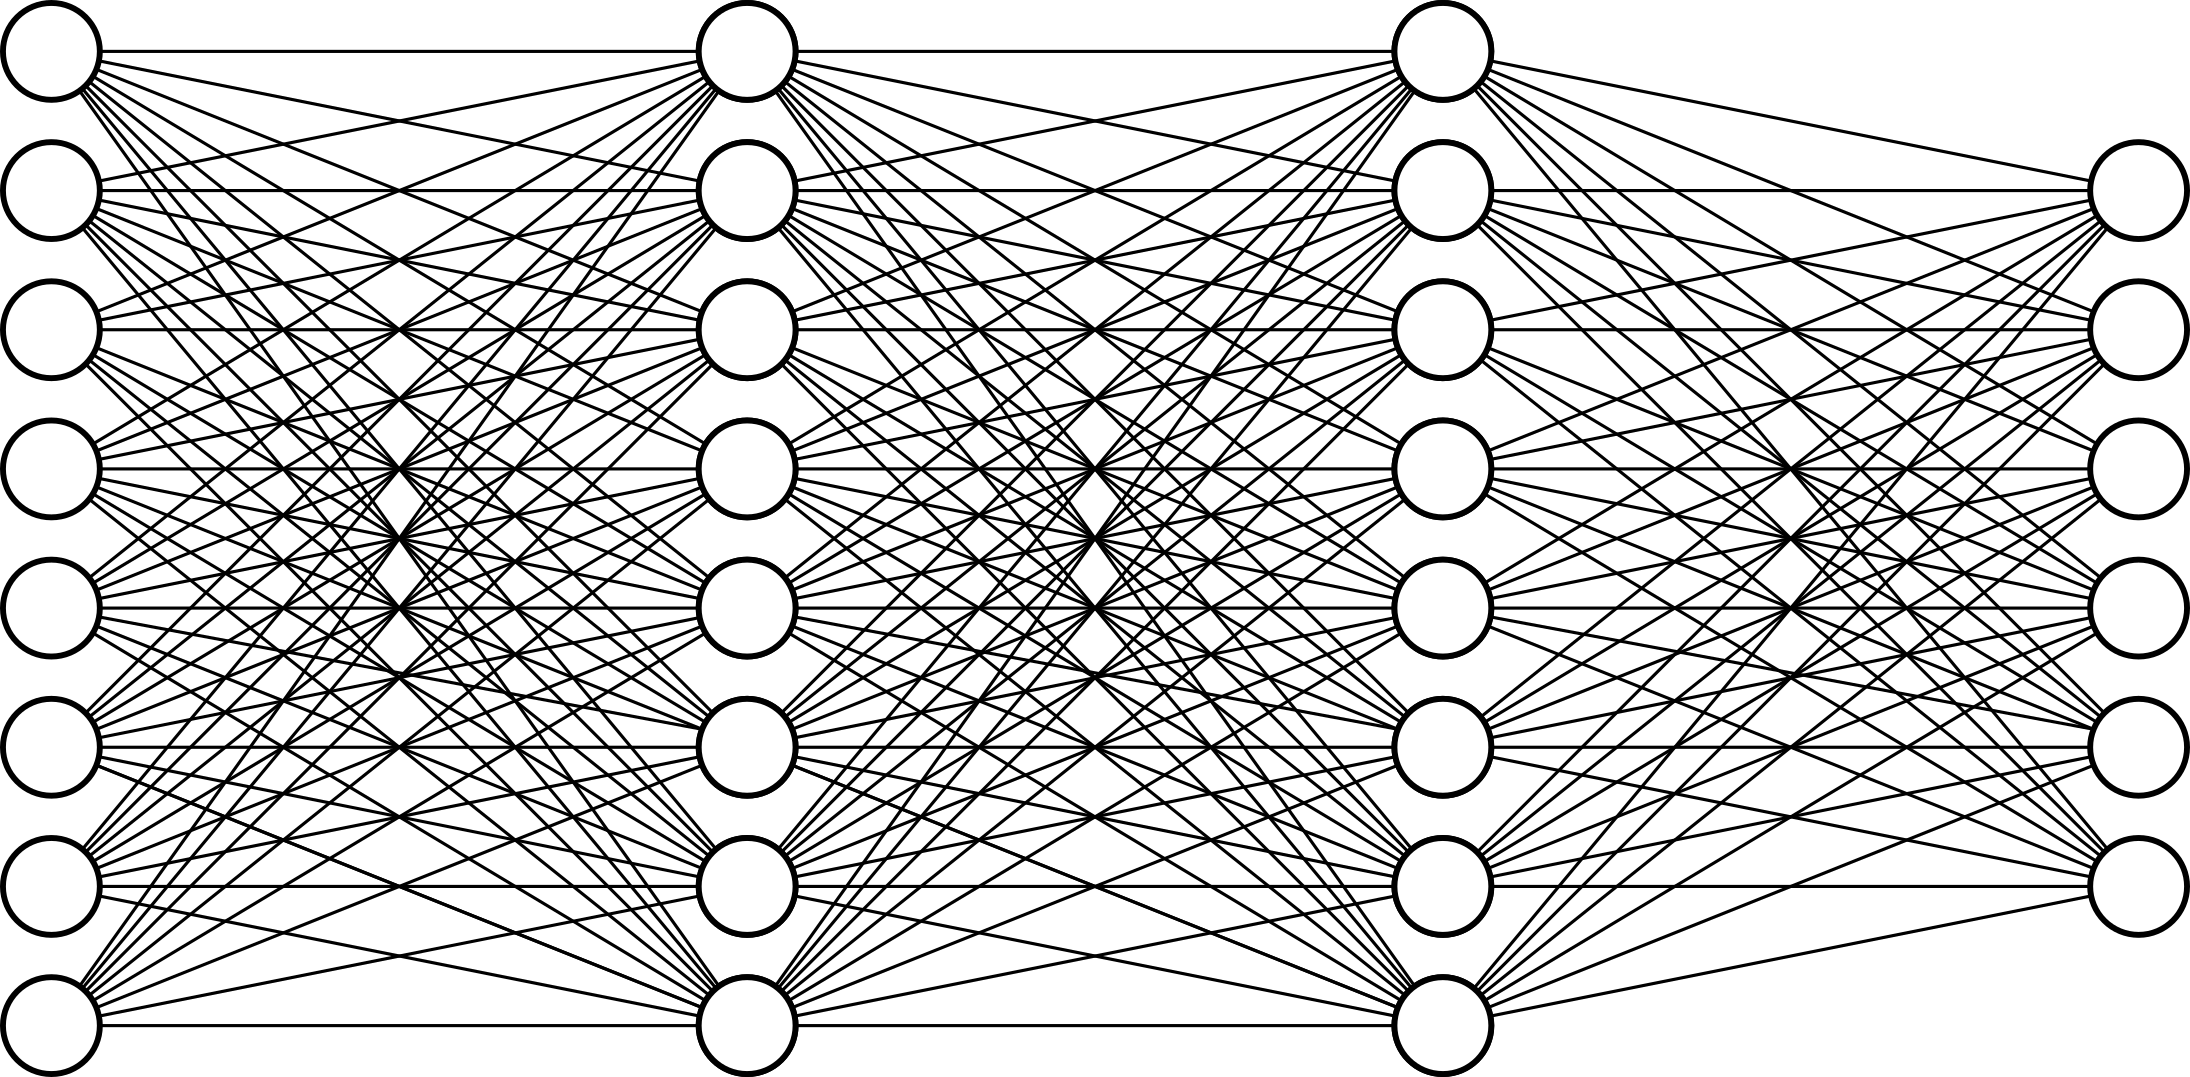
\includegraphics[height=3cm]{mini_reseau3_bis.png}
    \end{figure}
    \begin{figure}
      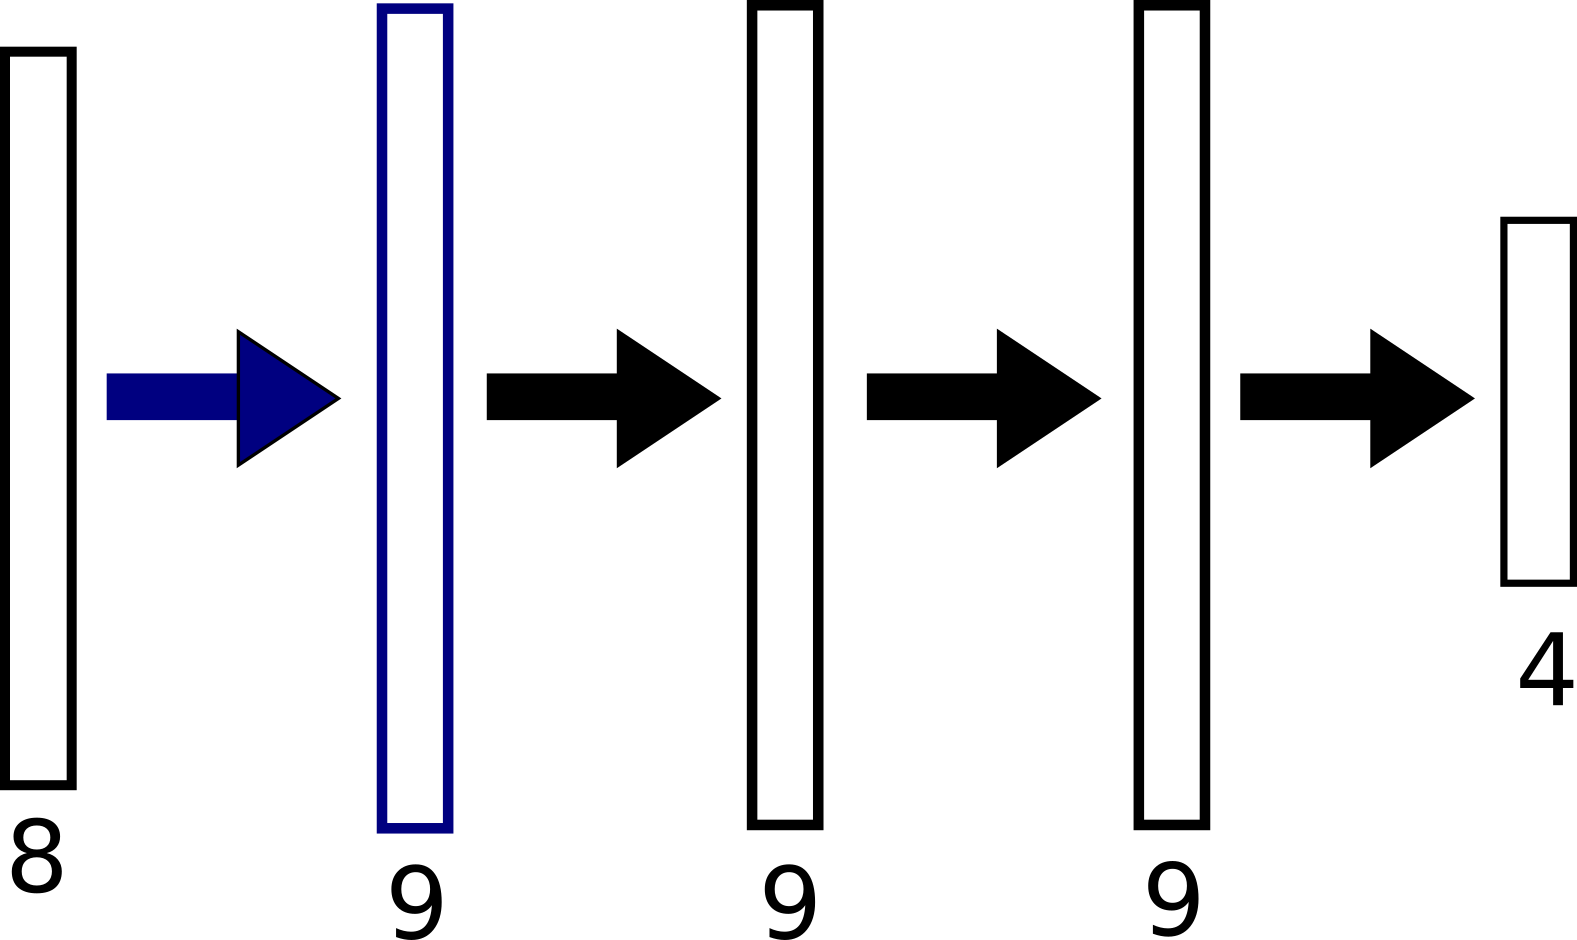
\includegraphics[height=3cm]{nn_representation}
    \end{figure}
  \end{column}

  \begin{column}{.5\textwidth}
    \begin{itemize}
    \item Data is organized into arrays, linked with operators
    \item A layer corresponds to an operator between arrays.
    \end{itemize}
  \end{column}
\end{columns}

\end{frame}


%%%%%%%%%%%%%%%%%%%%%%%%%%%%%%%%%%%%
\begin{frame}{The equations of fully-connected layers}

    \begin{figure}
      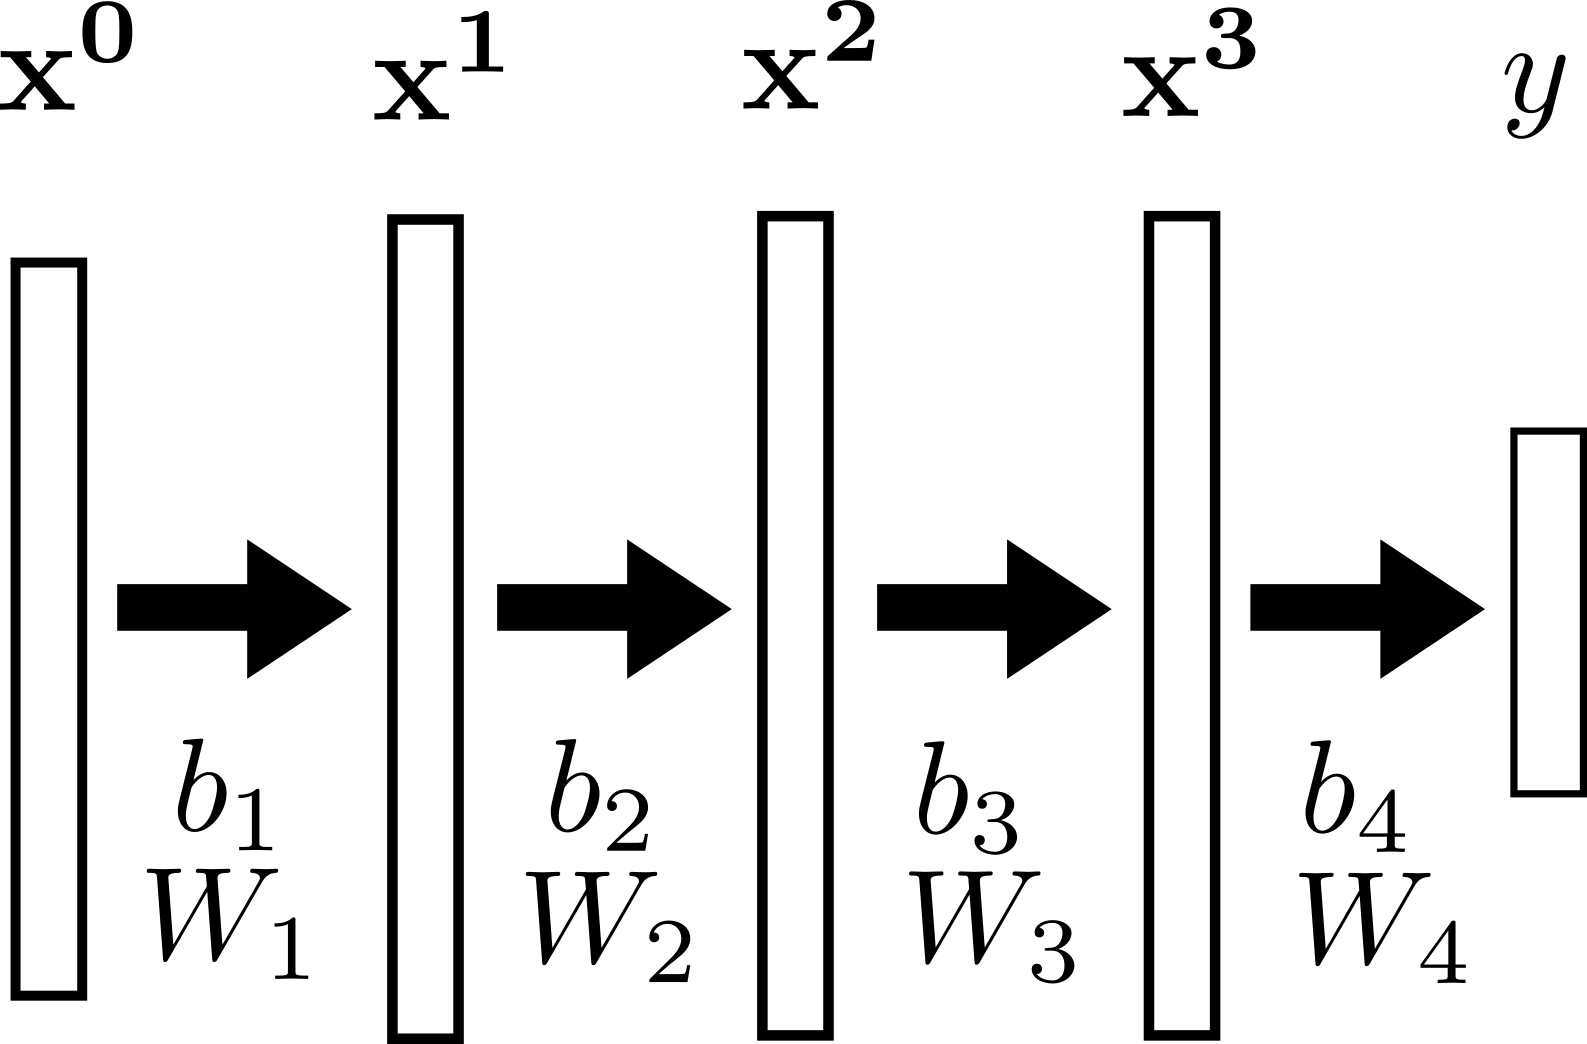
\includegraphics[height=3cm]{nn_representation2}
    \end{figure}

    \begin{block}{}
      \[\x^i = \act_i(\W_i\x^{i-1} + \bias_i),\, i= 1, 2, 3 \]
      \[y = \act_4(\W_4\x^4 + \bias_4)\]
    \end{block}

\end{frame}

%%%%%%%%%%%%%%%%%%%%%%%%%%%%%%%%%%%%%%%%%%%%%%%%%%

\frame{
  \frametitle{Activation: binary}

  \begin{columns}
    \begin{column}{.5\textwidth}
      \[
      \act(x)=
      \begin{cases}
        1,& \text{if } x > 0\\
        0,              & \text{otherwise}
      \end{cases}
      \]

    \end{column}

    \begin{column}{.5\textwidth}
      \begin{figure}
        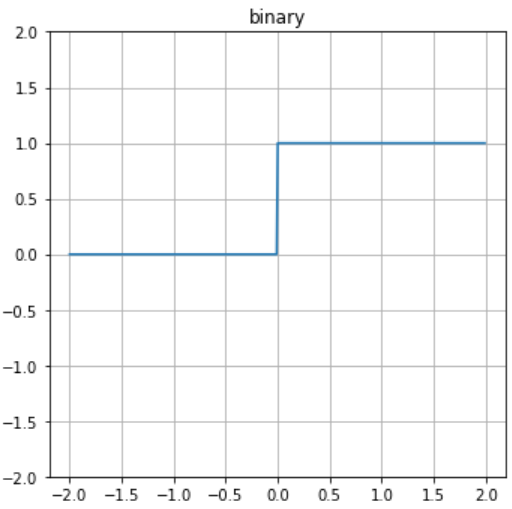
\includegraphics[width=.8\textwidth]{act_bin.png}
      \end{figure}


    \end{column}
  \end{columns}

  \begin{block}{Remarks}
    \begin{itemize}
    \item Biologically inspired
    \item[+] Simple to compute
    \item[+] High abstraction
    \item[-] Gradient nil except on one point
    \item \alert{In practice, almost never used}
    \end{itemize}
  \end{block}


}

%%%%%%%%%%%%%%%%%%%%%%%%%%%%%%%%%%%%%%%%%%%%%%%%%%

\frame{
  \frametitle{Activation: sigmoid}

  \begin{columns}
    \begin{column}{.5\textwidth}
      \[
      \act(x)= \frac{1}{1 + e^{-x}}
      \]
    \end{column}

    \begin{column}{.5\textwidth}
      \begin{figure}
        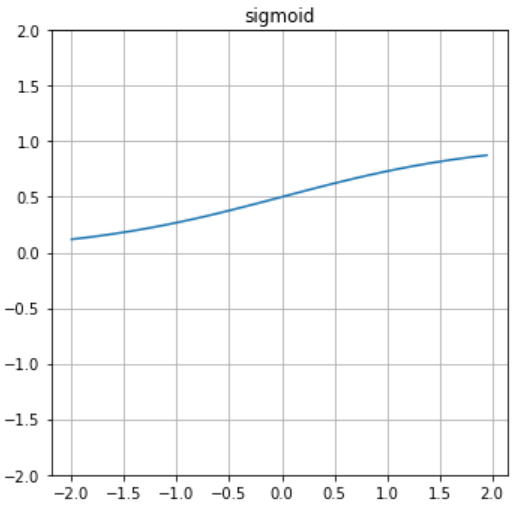
\includegraphics[width=.8\textwidth]{act_sigm.png}
      \end{figure}


    \end{column}
  \end{columns}

  \begin{block}{Remarks}
    \begin{itemize}
    \item[+] Similar to binary activation, but with usable gradient
    \item[-] However, gradient tends to zero when input is far from zero
    \item[-] More computationally intensive
    \end{itemize}
  \end{block}



}

%%%%%%%%%%%%%%%%%%%%%%%%%%%%%%%%%%%%%%%%%%%%%%%%%%

\frame{
  \frametitle{Activation: hyperbolic tangent}

  \begin{columns}
    \begin{column}{.5\textwidth}
      \[
      \act(x)= \frac{e^x - e^{-x}}{e^x + e^{-x}}
      \]
    \end{column}

    \begin{column}{.5\textwidth}
      \begin{figure}
        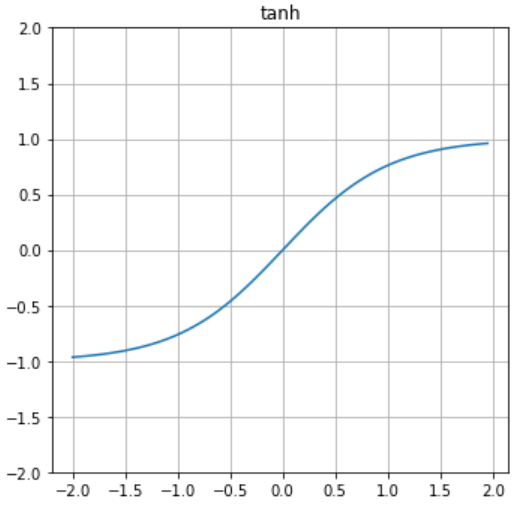
\includegraphics[width=.8\textwidth]{act_tanh.png}
      \end{figure}


    \end{column}
  \end{columns}

  \begin{block}{Remarks}
    \begin{itemize}
    \item Similar to sigmoid
    \end{itemize}
  \end{block}



}


%%%%%%%%%%%%%%%%%%%%%%%%%%%%%%%%%%%%%%%%%%%%%%%%%%

\frame{
  \frametitle{Activation: rectified linear unit (ReLU)}

  \begin{columns}
    \begin{column}{.5\textwidth}
      \[
      \act(x)=
      \begin{cases}
        x,& \text{if } x > 0\\
        0,              & \text{otherwise}
      \end{cases}
      \]
    \end{column}

    \begin{column}{.5\textwidth}
      \begin{figure}
        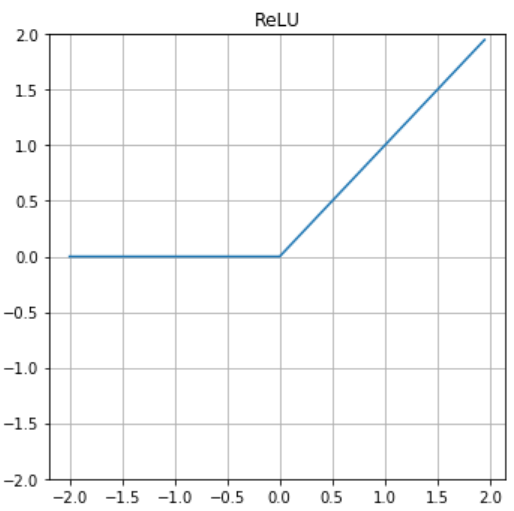
\includegraphics[width=.8\textwidth]{act_relu.png}
      \end{figure}


    \end{column}
  \end{columns}

  \begin{block}{Remarks}
    \begin{itemize}
    \item[+] Usable gradient when activated
    \item[+] Fast to compute
    \item[+] High abstraction
    \end{itemize}
  \end{block}

\pause

  \begin{alertblock}{}
    ReLU is the most commonly used activation function.
  \end{alertblock}


}


%%%%%%%%%%%%%%%%%%%%%%%%%%%%%%%%%%%%%%%%%%%%%%%%%%
\section{Learning with convolutional neural networks}
%%%%%%%%%%%%%%%%%%%%%%%%%%%%%%%%%%%%%%%%%%%%%%%%%%

%%%%%%%%%%%%%%%%%%%%%%%%%%%%%%%%%%%%%%%%%%%%%%%%%%
\begin{frame}{Machine Learning: basic definitions}
\begin{itemize}
	\item Machine Learning aims at predicting some output $y$ from an input (or measurement) $x$:
	\begin{equation}
	y = f(x)
	\end{equation}
	\item In this formulation, Machine Learning aims at finding (learning) $f$ from available data.
	\item The data that is used to learn $f$ is called \textbf{training set}, denoted by $\X$.
	\item In this general formulation, there is no particular limitation as to the mathematical nature of $x$ and $y$. Today, $x$ will be an image, and $y$ a class, a vector, or another image.
\end{itemize}
\end{frame}

\begin{frame}{A simple example: polynomial curve fitting\footnote{Example adapted from \cite{Bishop2006}}}
\begin{figure}[htb]
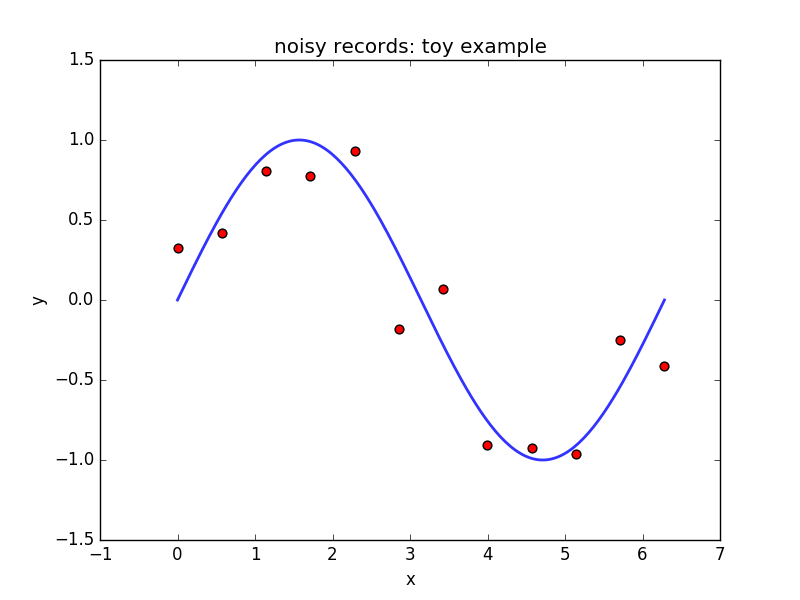
\includegraphics[width=0.6\textwidth]{../graphics/sample_from_sin.png}
\end{figure}
\begin{itemize}
	\item From a set of measured points $(x_i, y_i)$ (red), we would like to build a model to predict the value $y$ for any given $x$.
	\item The true function is $g(x)=\sin (x)$ (displayed in blue).
	\item The measurements $y_i$ are noisy outputs of that function, i.e.
	\begin{equation}
	y_i = \sin (x_i) + \epsilon \; , \;\;\; \;\;\; \epsilon \sim \mathcal{N}(0,0.2)
	\end{equation}
\end{itemize}
\end{frame}

\begin{frame}{A simple example: polynomial curve fitting}
\begin{itemize}
	\item We use the following polynomial model:
	\begin{eqnarray}
	f(x) &=& a_0 + a_1 x + a_2 x^2 + \ldots + a_m x^m \nonumber \\
	&=& \param^T \featmap (x)
	\end{eqnarray}
	\item Parameter vector: $\param = (a_0, a_1, \ldots, a_m)^T$
	\item Here, the initial measurement $x$ is a scalar. In our model, we map $x$ to a higher dimensional space:
	\begin{eqnarray}
		\featmap : \mathbb{R}^{\nfeatures} &\rightarrow & \mathbb{R}^Q \nonumber \\
		x &\rightarrow & \featmap (x) = (1, x, x^2, \ldots, x^m)^T
	\end{eqnarray}
	\item The model is linear in the parameters $\theta$ and linear in $\featmap$, but for $m>1$, the model is not linear in $x$.
\end{itemize}
\end{frame}

\begin{frame}{A simple example: polynomial curve fitting}
\begin{itemize}
	\item One classical approach is to minimize the least squared error between measured and predicted values:
	\begin{eqnarray}
		\min_{\param} \loss(\param) &=& \min_{\param} \sum_{i=1}^N (y_i - f(x_i))^2 \nonumber \\
		&=& \min_{\param} \sum_{i=1}^N (y_i - \param^T \featmap (x_i))^2
	\end{eqnarray}
	\item This can be achieved by setting the gradient with respect to $\param$ to zero:
	\begin{equation}
		\nabla_{\param} \loss = (\frac{\partial \loss}{\partial a_0}, \frac{\partial \loss}{\partial a_1}, \ldots, \frac{\partial \loss}{\partial a_m} )^T = 0
	\end{equation}
	\item Unlike most optimization problems in this course, this leads to an analytical solution for $\param$. This is known as \textbf{linear regression}. For more details, we refer to \cite{Hastie2009}.
\end{itemize}
\end{frame}

\begin{frame}{Overfitting and underfitting}
\begin{columns}
\begin{column}{.8\textwidth}
\begin{figure}[htb]
	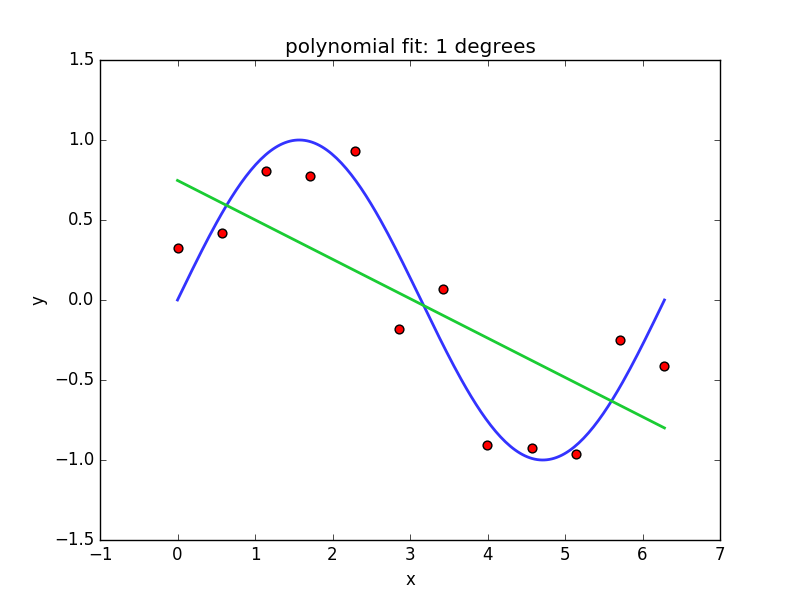
\includegraphics[width=0.75\textwidth]{../graphics/polyfit_degree_1.png}
\end{figure}
\end{column}
\begin{column}{.2\textwidth}
$\| \param \|^2 = 0.67$
\end{column}
\end{columns}
For $m=1$, the model is linear in its inputs. The solution is not capable of modeling the measured data points; we get a poor approximation of the original function. The family of functions we have used was not complex enough to model the true data distribution. We also speak of \textbf{underfitting}.
%\begin{textblock}{0}(.9\textwidth,\paperheight)
%  Test
% \end{textblock}
\end{frame}

\begin{frame}{Overfitting and underfitting}
\begin{columns}
\begin{column}{.8\textwidth}
\begin{figure}[htb]
	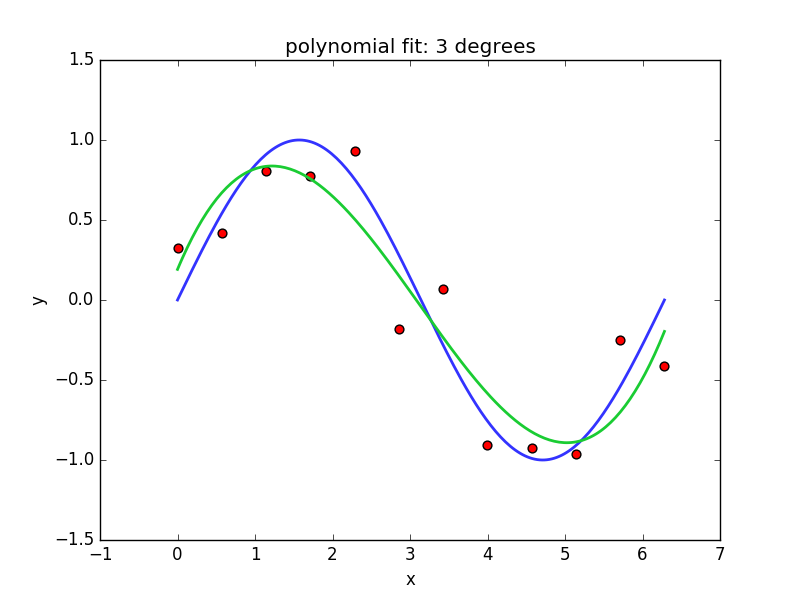
\includegraphics[width=0.75\textwidth]{../graphics/polyfit_degree_3.png}
\end{figure}
\end{column}
\begin{column}{.2\textwidth}
$\| \param \|^2 = 1.72$
\end{column}
\end{columns}
For $m=3$, we obtain a solution that seems to be quite right: it is sufficiently complex to model the true data distribution, but not too complex to model the small variations which are due to noise.
\end{frame}

\begin{frame}{Overfitting and underfitting}
\begin{columns}
\begin{column}{.8\textwidth}
\begin{figure}[htb]
	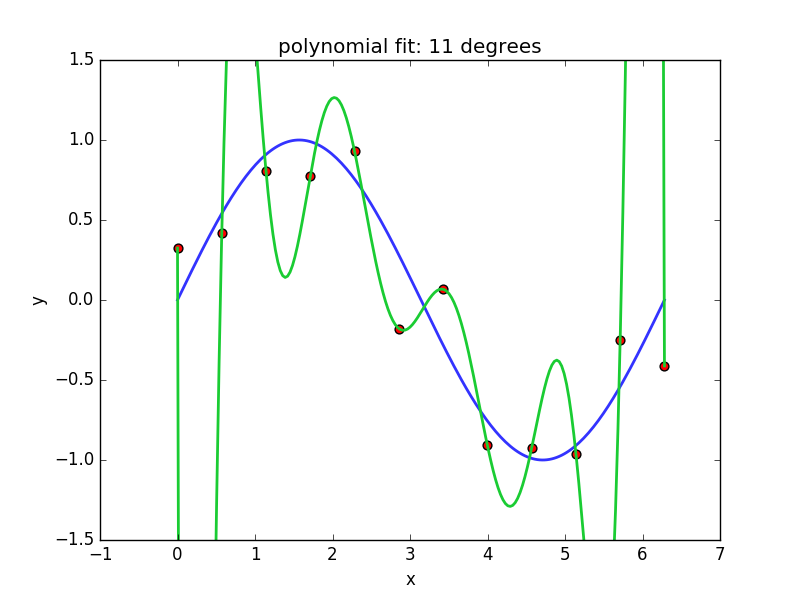
\includegraphics[width=0.75\textwidth]{../graphics/polyfit_degree_11.png}
\end{figure}
\end{column}
\begin{column}{.2\textwidth}
$\| \param \|^2 \approx 10^7$
\end{column}
\end{columns}
For $m=11$, we obtain a solution that has zero error (the function passes through every point of the training set). But the coefficients with large absolute values that cancel each other precisely on the training points lead to a highly unstable function. We speak of \textbf{overfitting} and \textbf{poor generalization}.
\end{frame}

\begin{frame}{Overfitting and underfitting}
\begin{columns}
\begin{column}{.8\textwidth}
\begin{figure}[htb]
	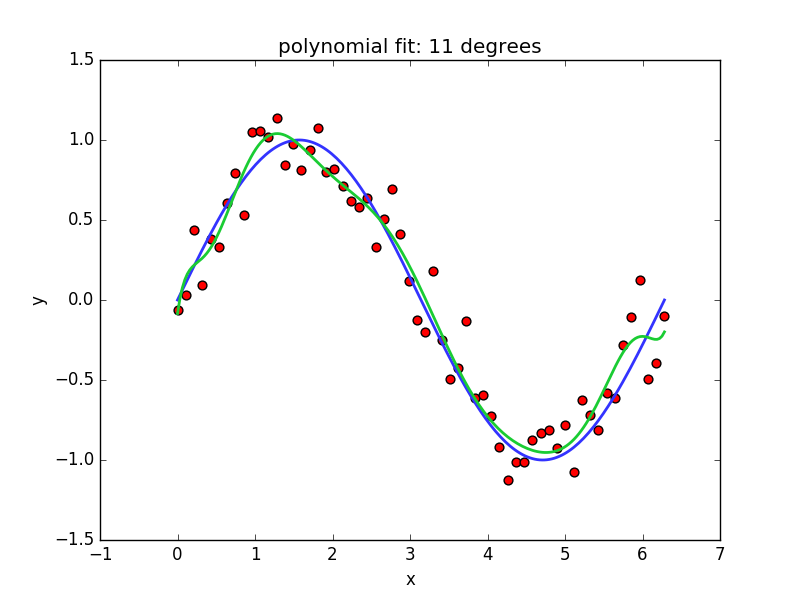
\includegraphics[width=0.75\textwidth]{../graphics/polyfit_degree_11_N60.png}
\end{figure}
\end{column}
\begin{column}{.2\textwidth}
$\| \param \|^2 = 5647$
\end{column}
\end{columns}
One way of reducing overfitting is to increase the number of samples. Even if the function is complex, it cannot be “too wild”, as it has to find a compromise between many training samples. This however implies the annotation (or measurement) of more samples.
\end{frame}

\begin{frame}{Overfitting and underfitting}
\begin{columns}
\begin{column}{.8\textwidth}
\begin{figure}[htb]
	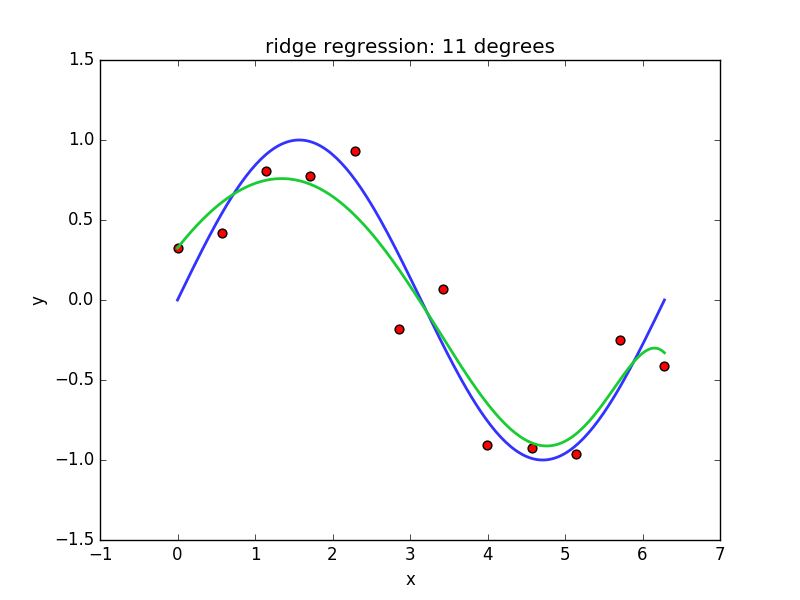
\includegraphics[width=0.75\textwidth]{../graphics/ridge_regression_11_10.png}
\end{figure}
\end{column}
\begin{column}{.2\textwidth}
$\| \param \|^2 = 0.41$
\end{column}
\end{columns}
Another way of preventing overfitting without increasing the number of samples, is to add a penalization term in the optimization procedure. This is also known as \textbf{regularization}:
\begin{equation}
	\loss = \sum_{i=1}^N (y_i - \param^T \featmap (x_i))^2 + \lambda \| \param \|^2
\end{equation}
\end{frame}


%%%%%%%%%%%%%%%%%%%%%%%%%%%%%%%%%%%%
\begin{frame}{A picture is worth a thousand words}

  \begin{columns}
    \begin{column}{.5\textwidth}
      \begin{block}{Definition}
        \begin{itemize}
        \item Classically, an image is a matrix of values belonging to $[0, \ldots, 255]$ (grey level images) or to $[0, \ldots, 255]^3$ (color images).
        \item More generally, an image is a $q$-dimensional array of values belonging to $R^d$.
        \end{itemize}
      \end{block}

    \end{column}

    \begin{column}{.5\textwidth}
      \begin{figure}
        \centering
        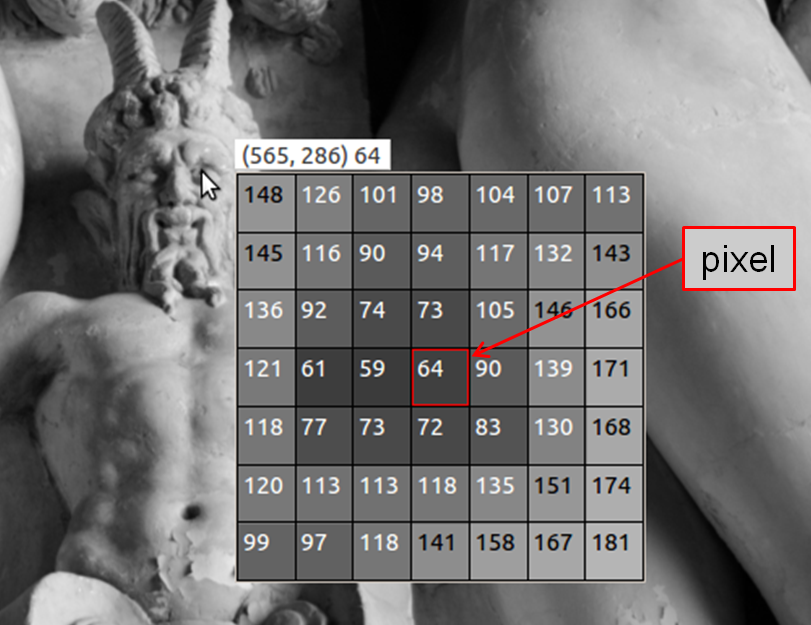
\includegraphics[width=5cm]{faune.png}\\
        \tiny{Grey level values around the left eye of the faun}
      \end{figure}

    \end{column}
  \end{columns}

\end{frame}


%%%%%%%%%%%%%%%%%%%%%%%%%%%%%%%%%%%%
\begin{frame}{The role of annotated image databases}

  Image databases including \emph{annotations} (typically some kind of high level information) are essential to the development of \emph{supervised} machine learning methods for image analysis.

  \begin{block}{Annotations}
    \begin{itemize}
    \item Image class
    \item Measure(s) obtained from the image
    \item Position of objects within the image
    \item Segmentation
    \end{itemize}
  \end{block}

\end{frame}

%%%%%%%%%%%%%%%%%%%%%%%%%%%%%%%%%%%%
\begin{frame}{MNIST database \tiny{\cite{lecun_gradient-based_1998}}}

  \begin{itemize}
  \item The Modified National Institute of Standards and Technology (MNIST) database contains $60\,000$ training images of hand-written digits, and $10,000$ test images.
  \item Image size: $28 \times 28$
  \item It has been used since 1998
  \item Human performance on a similar database (NIST) is reported to be around $1.5\%$ error \cite{simard_efficient_1993}
  \item Best methods, based on convolutional neural networks, give around $0.21\%$ test error.
  \end{itemize}

\end{frame}

%%%%%%%%%%%%%%%%%%%%%%%%%%%%%%%%%%%%
\begin{frame}{MNIST database}

  \centering
  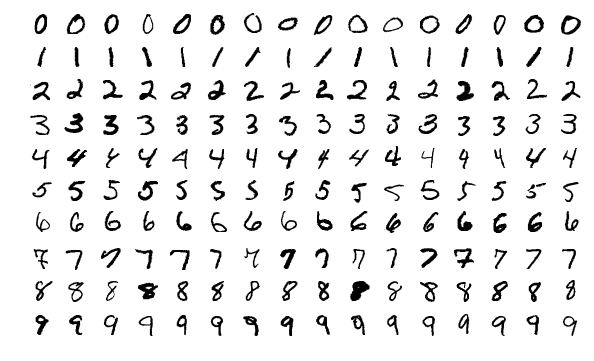
\includegraphics[width=\textwidth]{mnist_examples.png}\\
  \source{Images from MNIST assembled by Josef Stepan (licensed under CC BY-SA 4.0)}


\end{frame}



%%%%%%%%%%%%%%%%%%%%%%%%%%%%%%%%%%%%
\begin{frame}{Layers representation}

  \begin{block}{}
    For illustration purposes, in the following slides images and filters will be displayed as rows of neurons -- these can be seen as 1D arrays or as sections of 2D arrays.

    We represent some connections between neurons. Each such connection is associated to a weight. The bias are not represented, to avoid clutter, but must not be forgotten.
  \end{block}

  \begin{columns}

    \begin{column}<1->{0.33\textwidth}
      \begin{center}
        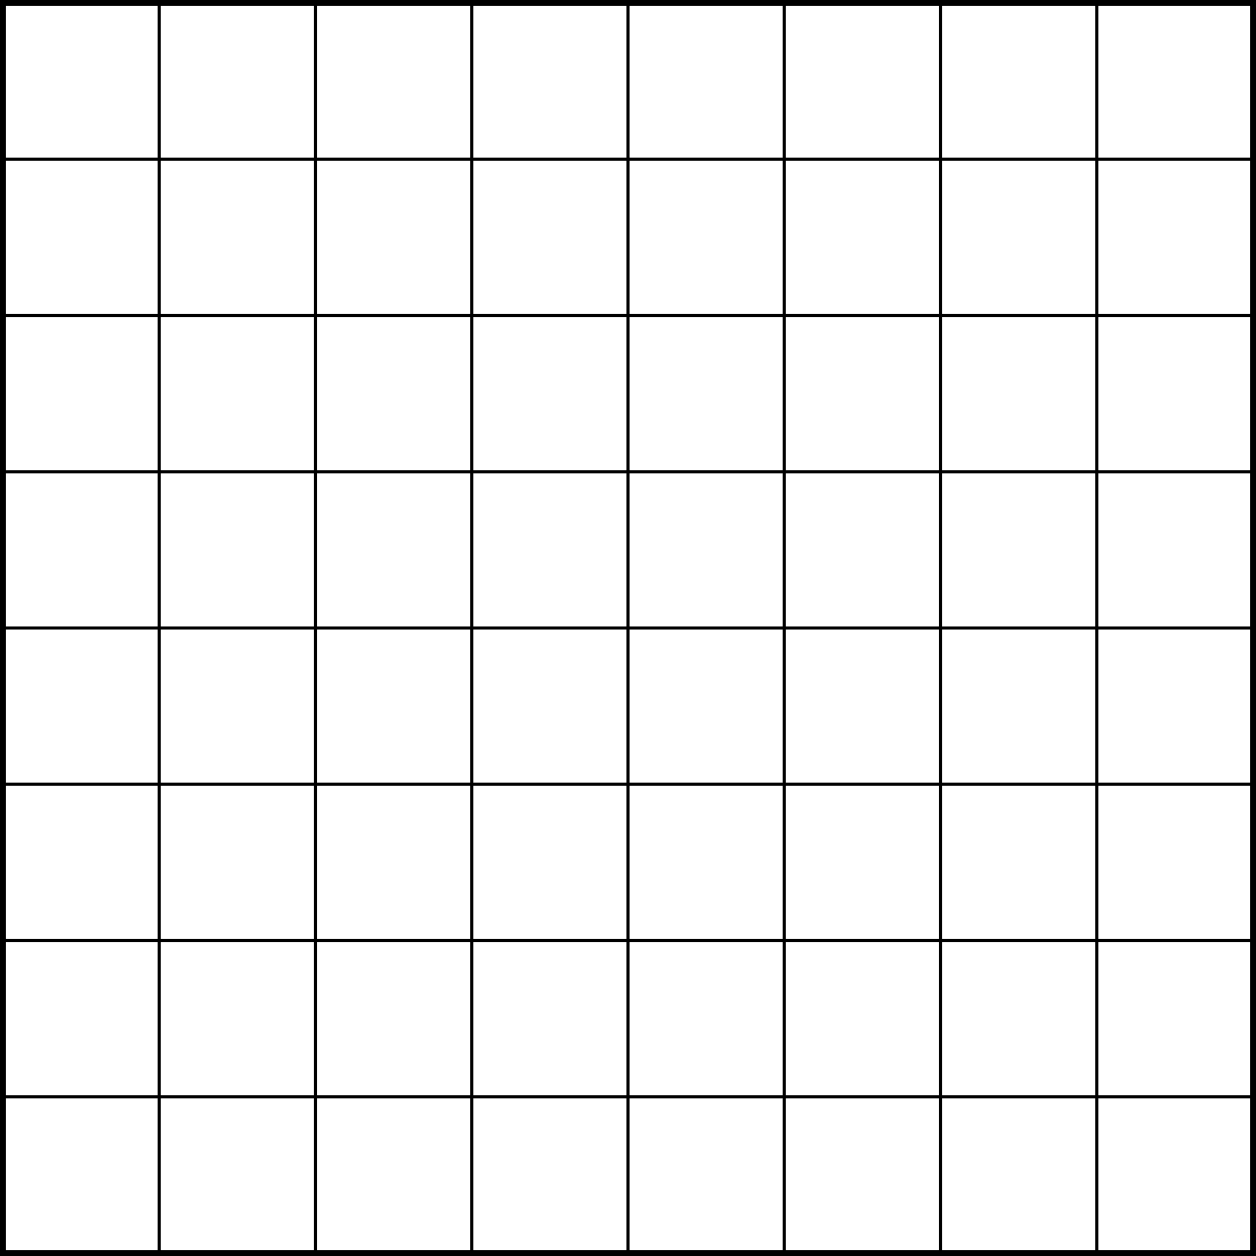
\includegraphics[width=0.80\textwidth]{cnn_pixels.png}
      \end{center}
    \end{column}

    \begin{column}<2->{0.33\textwidth}
      \begin{center}
        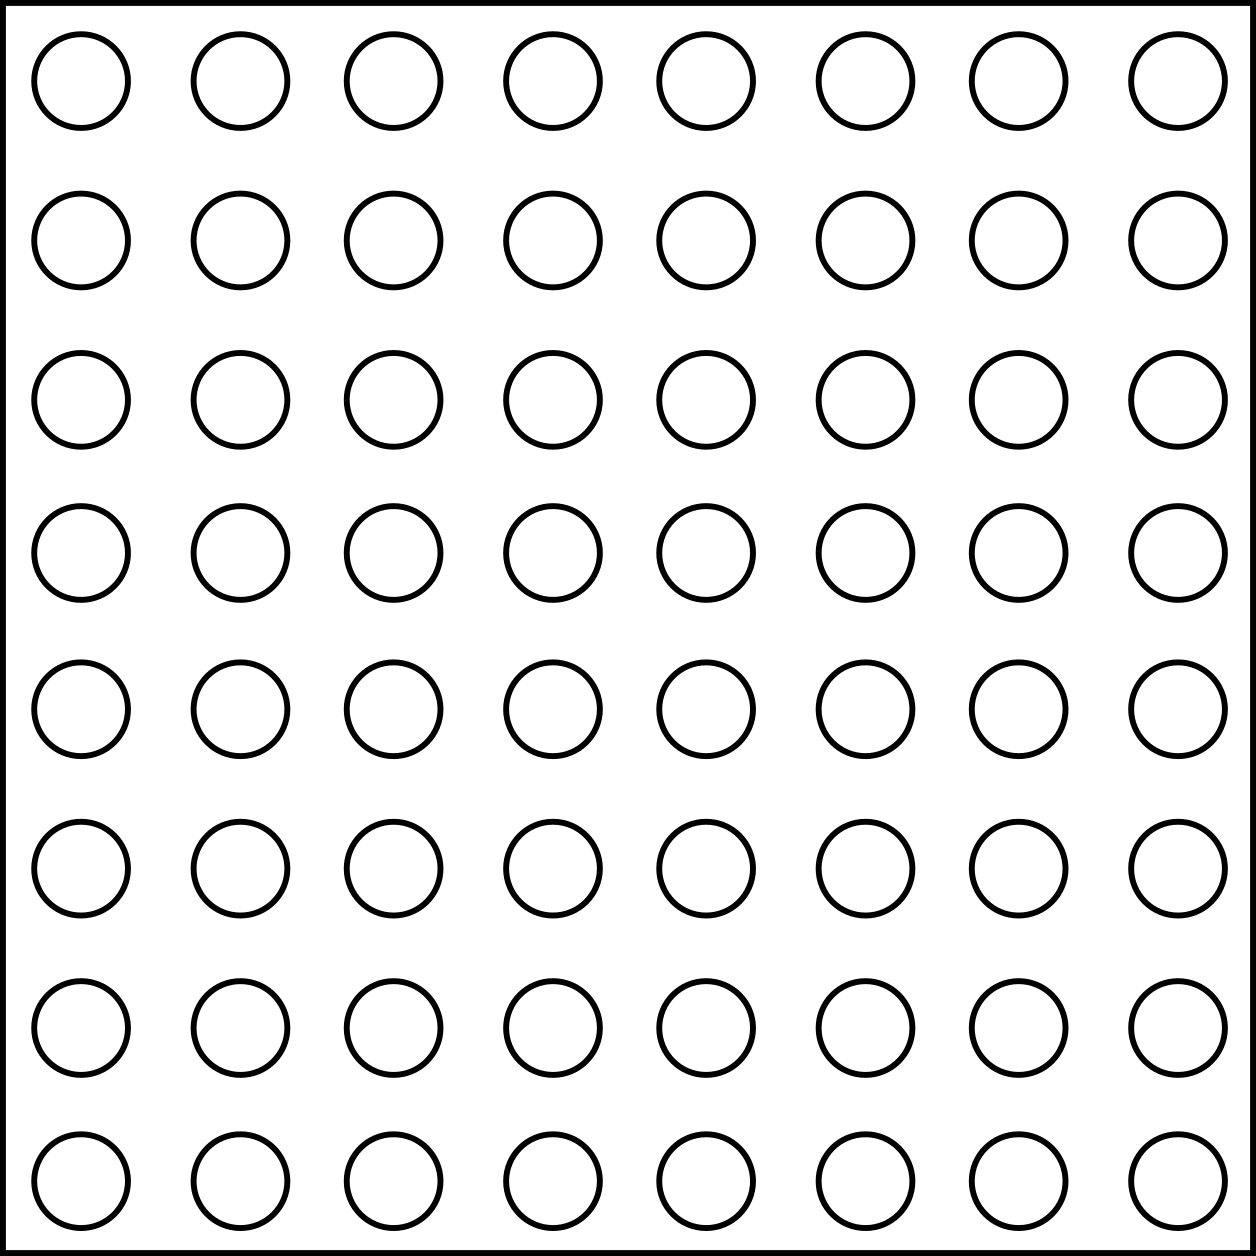
\includegraphics[width=0.80\textwidth]{cnn_neurones.png}

      \end{center}
    \end{column}

    \begin{column}<3->{0.33\textwidth}
      \begin{center}
        
\includegraphics[width=0.07\textwidth]{col.png}

      \end{center}
    \end{column}

  \end{columns}


\end{frame}


%%%%%%%%%%%%%%%%%%%%%%%%%%%%%%%%%%%%%%%%%%%%%%%%%%
\frame{
  \frametitle{Towards convolutional layers}


  \begin{columns}

    \begin{column}<1->{0.3\textwidth}
      \begin{center}
        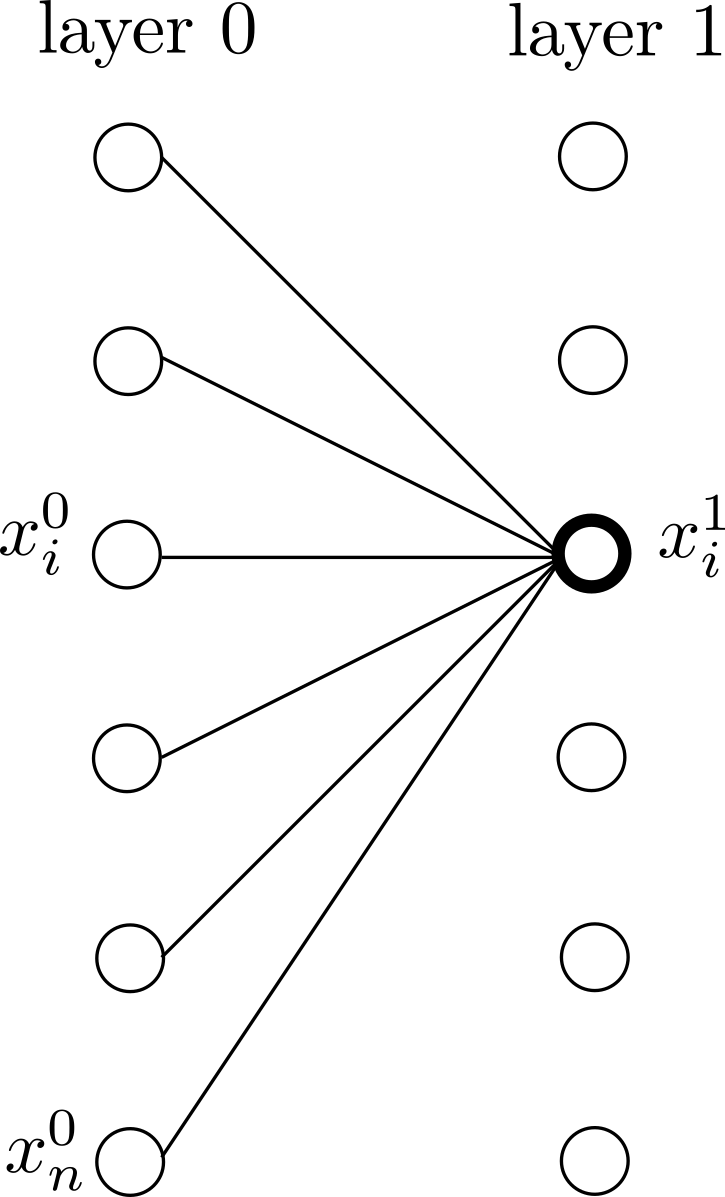
\includegraphics[width=0.74\textwidth]{fully_connected_layer.png}
        \\ \scriptsize{Fully connected layer: $n(n+1)$ weights}
      \end{center}
    \end{column}

    \begin{column}<2->{0.3\textwidth}
      \begin{center}
        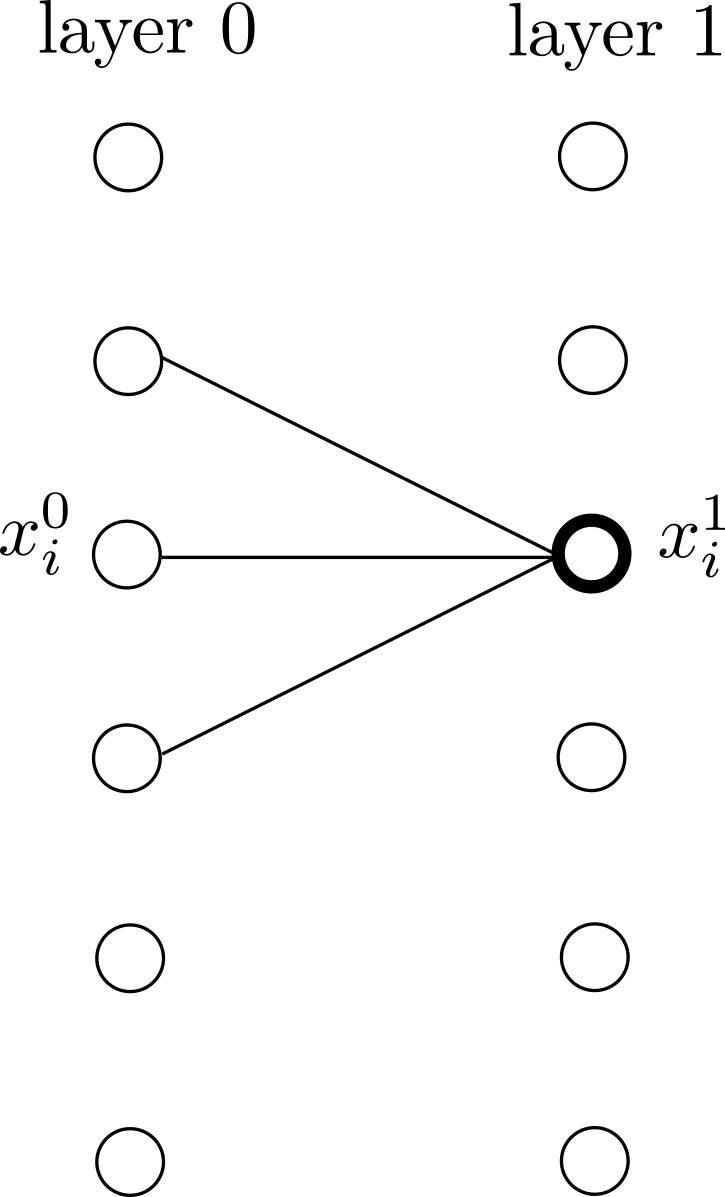
\includegraphics[width=0.74\textwidth]{locally_connected_layer.png}
        \\ \scriptsize{Locally conn. layer: $n(s+1)$ weights}
      \end{center}
    \end{column}

    \begin{column}<3->{0.3\textwidth}
      \begin{center}
        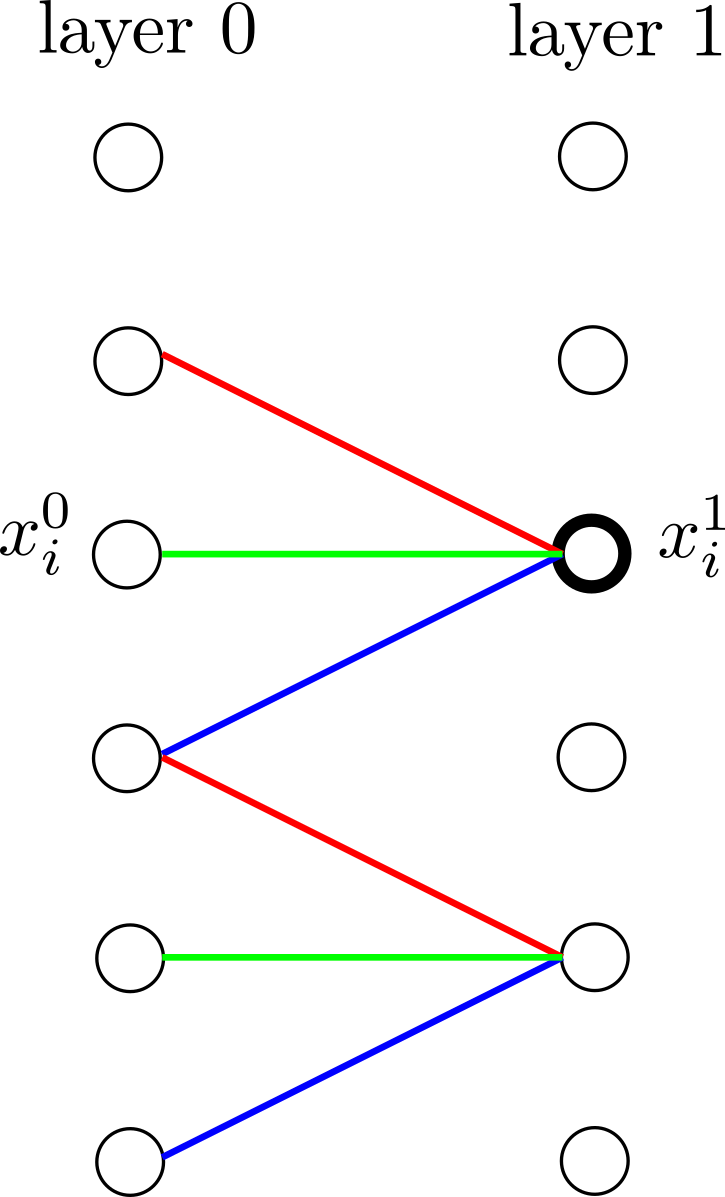
\includegraphics[width=0.74\textwidth]{convolutional_layer.png}
        \\ \scriptsize{Weight replication: $s+1$ weights.\\
          \alert{Convolutional layer.}}
      \end{center}
    \end{column}

  \end{columns}

}


%%%%%%%%%%%%%%%%%%%%%%%%%%%%%%%%%%%%%%%%%%%%%%%%%%
\frame{
  \frametitle{Towards convolutional layers: some figures}

  \begin{itemize}
  \item $3 \times 3$ convolutions: $s=9$
  \item \textcolor{blue}{Toy image: $n = 28 \times 28 = 784$}
  \item \textcolor{orange}{Typical image: $n = 1000 \times 1000 = 10^6$}
  \end{itemize}

  \begin{columns}

    \begin{column}{0.3\textwidth}
      \begin{center}
        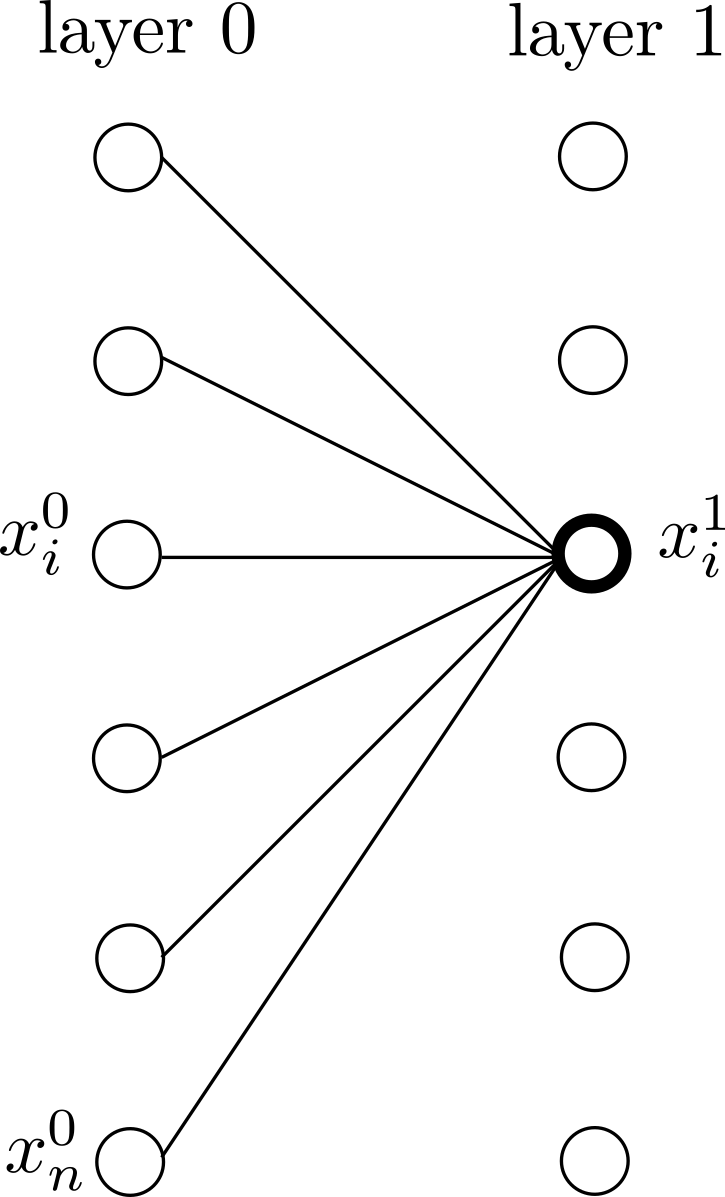
\includegraphics[width=0.74\textwidth]{fully_connected_layer.png}
        \\ \scriptsize{Fully connected layer: $n(n+1)$ weights}
        \\ \textcolor{blue}{\scriptsize{$\approx 6.10^5$}}
        \\ \textcolor{orange}{\scriptsize{$\approx 10^{12}$}}
      \end{center}
    \end{column}

    \begin{column}{0.3\textwidth}
      \begin{center}
        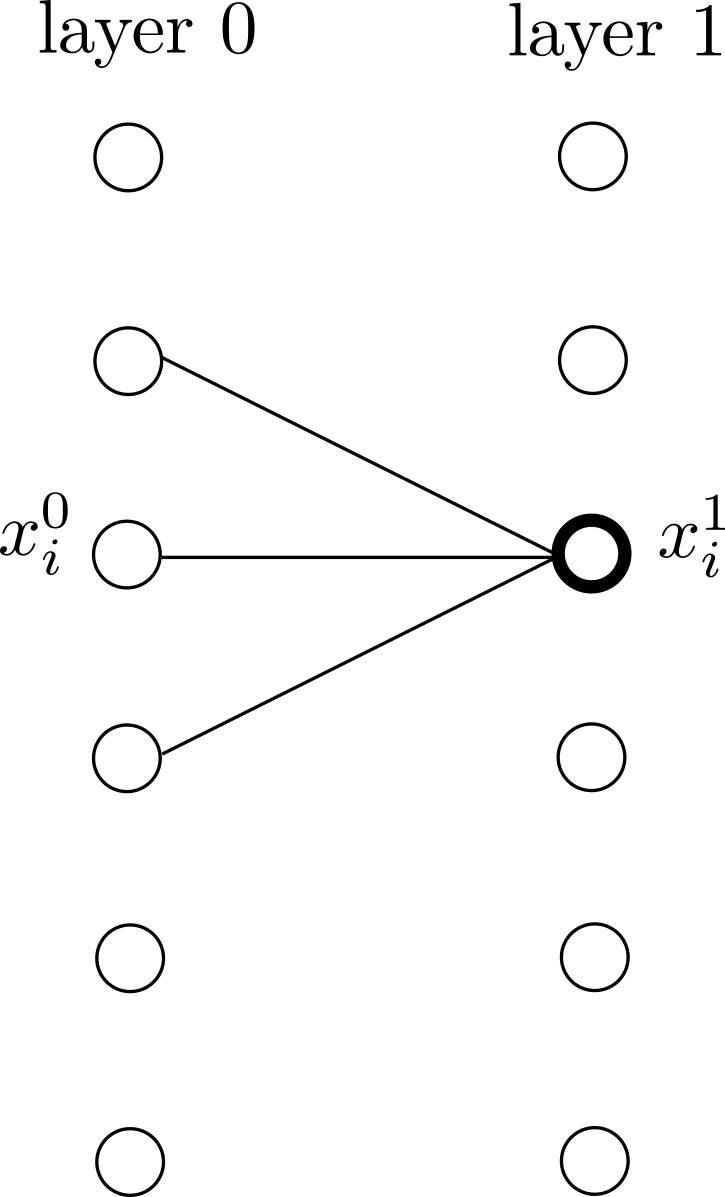
\includegraphics[width=0.74\textwidth]{locally_connected_layer.png}
        \\ \scriptsize{Locally conn. layer: $n(s+1)$ weights}
        \\ \textcolor{blue}{\scriptsize{$7840$}}
        \\ \textcolor{orange}{\scriptsize{$10^7$}}
      \end{center}
    \end{column}

    \begin{column}{0.3\textwidth}
      \begin{center}
        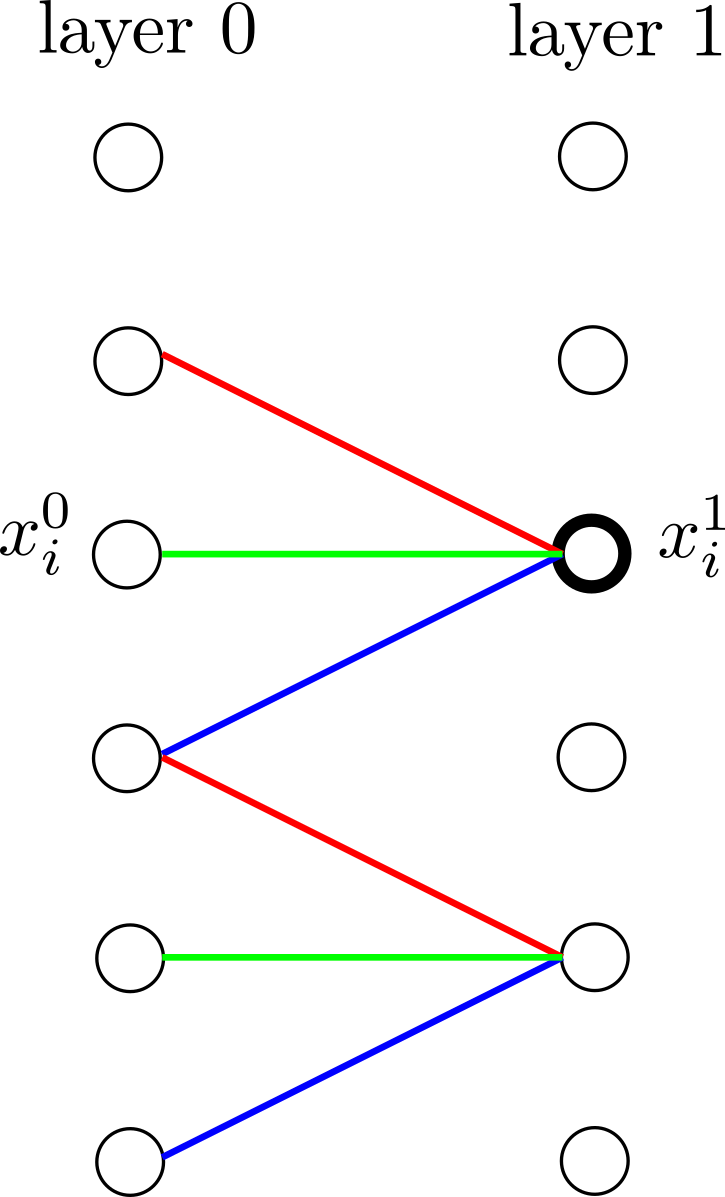
\includegraphics[width=0.74\textwidth]{convolutional_layer.png}
        \\ \scriptsize{Weight replication: $s+1$ weights.}
        \\ \textcolor{blue}{\scriptsize{$10$}}
        \\ \textcolor{orange}{\scriptsize{$10$}}

      \end{center}
    \end{column}

  \end{columns}
}


%%%%%%%%%%%%%%%%%%%%%%%%%%%%%%%%%%%%
\begin{frame}{Convolutional layer illustration in 2D}


  \begin{itemize}
  \item Illustration of a convolution of size $3 \times 3$
  \end{itemize}

  \begin{center}
    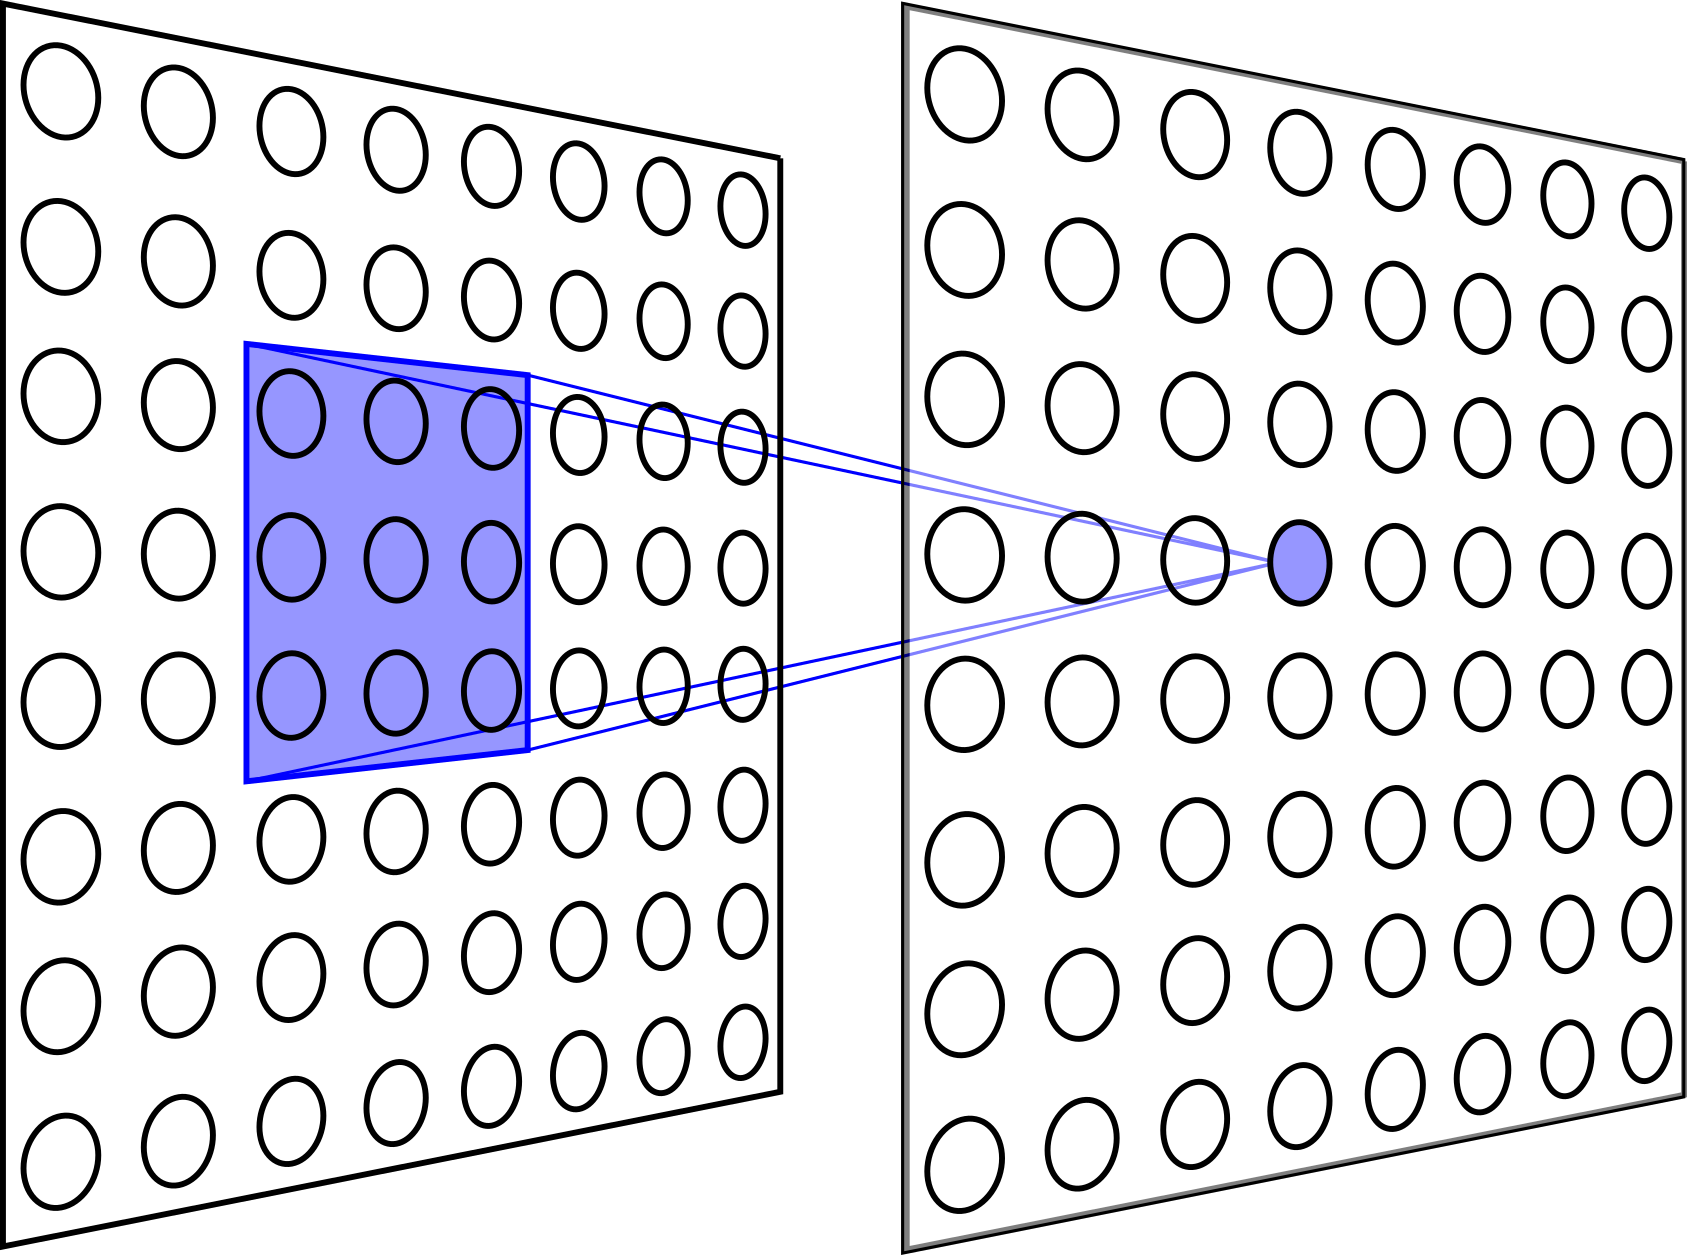
\includegraphics[width=0.5\textwidth]{cnn_complet}
  \end{center}


\end{frame}

%%%%%%%%%%%%%%%%%%%%%%%%%%%%%%%%%%%%%%%%%%%%%%%%%%
\frame{
  \frametitle{Stride}

  A convolutional layer can at the same time downsample the image by applying a sampling step, or \emph{stride}.

  \begin{columns}

    \begin{column}<1->{0.3\textwidth}
      \begin{center}
        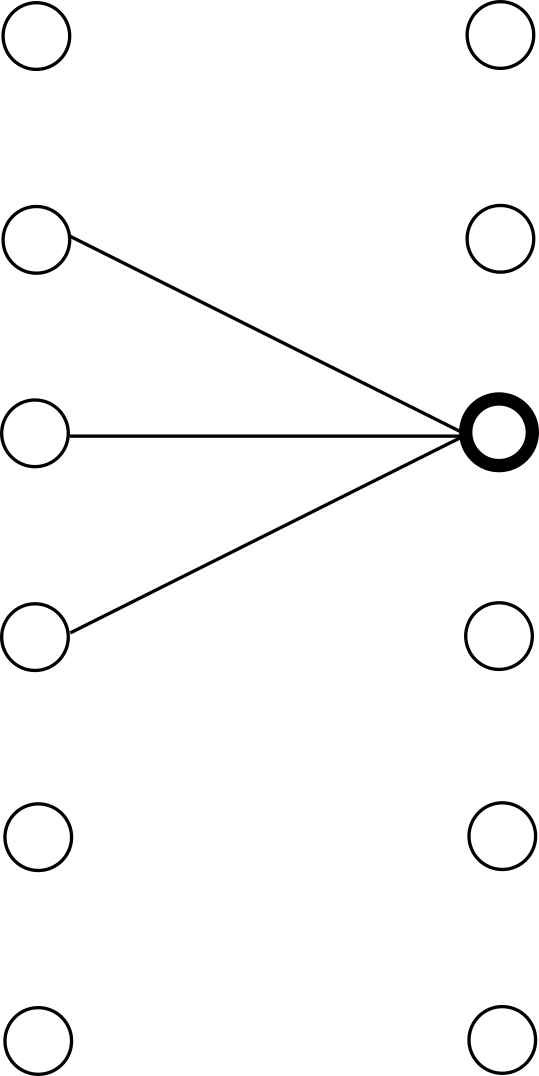
\includegraphics[width=0.60\textwidth]{stride1.png}
        \\ \scriptsize{Stride 1}
      \end{center}
    \end{column}

    \begin{column}<2->{0.3\textwidth}
      \begin{center}
        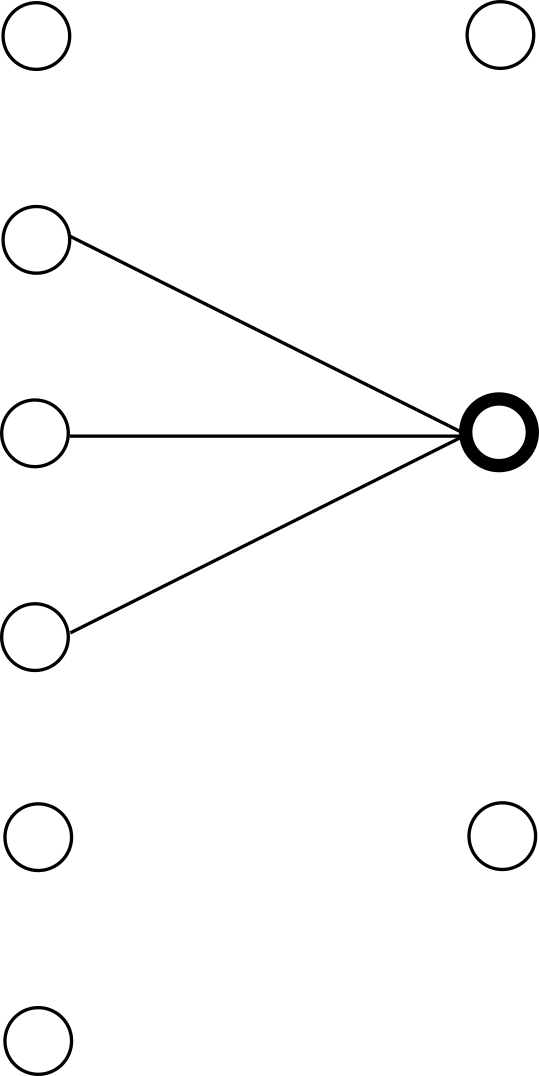
\includegraphics[width=0.60\textwidth]{stride2.png}
        \\ \scriptsize{Stride 2}
      \end{center}
    \end{column}

    \begin{column}<3>{0.3\textwidth}
      \begin{center}
        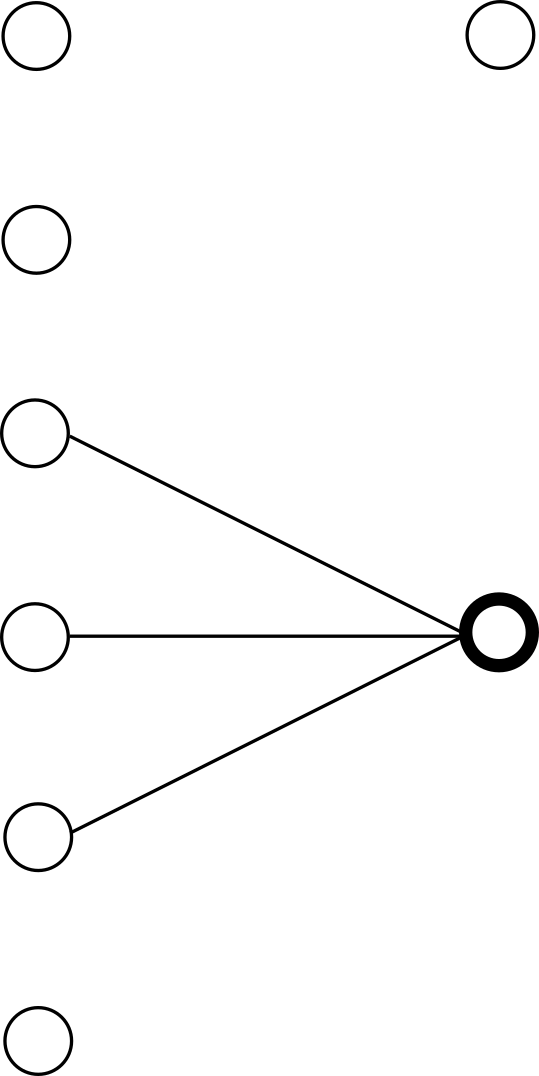
\includegraphics[width=0.60\textwidth]{stride3.png}
        \\ \scriptsize{Stride 3}
      \end{center}
    \end{column}

  \end{columns}

}

%%%%%%%%%%%%%%%%%%%%%%%%%%%%%%%%%%%%%%%%%%%%%%%%%%
\frame{
  \frametitle{Several filters in the same convolutional layer}


\begin{columns}
  \begin{column}{.53\textwidth}
  \begin{center}
    \includegraphics[width=\textwidth]{convolutional_layer2.png}
  \end{center}

  \end{column}

  \begin{column}{.47\textwidth}
\begin{block}{Note on vocabulary}
  The depth of a layer is often called the \alert{number of filters}.
\end{block}
  \end{column}
\end{columns}



}

%%%%%%%%%%%%%%%%%%%%%%%%%%%%%%%%%%%%%%%%%%%%%%%%%%
\frame{
  \frametitle{Several filters in the same convolutional layer}

  \begin{center}
    \includegraphics[width=0.53\textwidth]{convolutional_layer3.png}

  \end{center}


}

%%%%%%%%%%%%%%%%%%%%%%%%%%%%%%%%%%%%%%%%%%%%%%%%%%
\frame{
  \frametitle{Several filters in the same convolutional layer}

  \begin{center}
    \includegraphics[width=0.53\textwidth]{convolutional_layer4.png}

  \end{center}


}

%%%%%%%%%%%%%%%%%%%%%%%%%%%%%%%%%%%%
\begin{frame}{Branch merging: concatenation}

  \begin{center}
    \includegraphics[width=0.5\textwidth]{concatenation.png}
  \end{center}

\end{frame}


%%%%%%%%%%%%%%%%%%%%%%%%%%%%%%%%%%%%
\begin{frame}{1D representations}

  \centering
  \includegraphics[width=\textwidth]{fovea_convnet2}

  \vspace{1em}
  \pause

  \begin{columns}
    \begin{column}{.5\textwidth}
      \includegraphics[width=0.8\textwidth]{Fundus_photograph_of_normal_right_eye.jpg}
    \end{column}
    \begin{column}{.5\textwidth}
      This NN was used to estimate the position of the center of the macula on fundus images.
    \end{column}
  \end{columns}

  \source{NN is work of Robin Alais et al.\\Fundus image by Mikael Häggström, used with permission (CC0).}


\end{frame}

%%%%%%%%%%%%%%%%%%%%%%%%%%%%%%%%%%%%
\begin{frame}{2D representations}

  \begin{center}
    \begin{figure}
      \includegraphics[width=0.75\textwidth]{vgg16.png}
      \source{VGG16 (From https://www.cs.toronto.edu/~frossard/post/vgg16/)}
    \end{figure}
  \end{center}

\end{frame}

%%%%%%%%%%%%%%%%%%%%%%%%%%%%%%%%%%%%%%%%%%%%%%%%%%
\frame{
  \frametitle{U-Net architecture \cite{ronneberger_u-net:_2015}}

  \begin{figure}
    \includegraphics[width=0.95\textwidth]{unet_lo}
  \end{figure}

}



%%%%%%%%%%%%%%%%%%%%%%%%%%%%%%%%%%%%
\begin{frame}{Example: counting cells}

    \begin{figure}
      \includegraphics[width=\textwidth]{lazard0}
      \source{Tristan Lazard, master thesis. In collaboration with L'Oréal.}
    \end{figure}

\end{frame}


%%%%%%%%%%%%%%%%%%%%%%%%%%%%%%%%%%%%
\begin{frame}<beamer>{Counting cells}

    \begin{figure}
      \includegraphics[width=\textwidth]{lazard}
      \source{Tristan Lazard, master thesis. In collaboration with L'Oréal.}
    \end{figure}

\end{frame}

%%%%%%%%%%%%%%%%%%%%%%%%%%%%%%%%%%
\section{Autoencoders and generative adversarial networks}
%%%%%%%%%%%%%%%%%%%%%%%%%%%%%%%%%%

%%%%%%%%%%%%%%%%%%%%%%%%%%%%%%%%%%
\begin{frame}%{Reminder of Machine Learning Problems}
%\begin{enumerate}
{Supervised Learning} Given a labeled dataset $(\X,\mathbf{Y})$, we would like to learn a mapping from data space to label space.
\begin{figure}
\centering
\begin{tikzpicture}
\tikzstyle{main}=[circle, minimum size = 6mm, thick, draw =black!80, node distance = 26mm]
\tikzstyle{connect}=[-latex, thick]
  \node[main, fill = white!50] (alpha) [label=below: $\x$] {\includegraphics[width=.15\columnwidth]{Animal}};
  \node[main,fill = red!50] (xout) [right= of alpha,label=below: What animal is this?] {$\hat{\y} \in \mathbb{Z}$ };
  \draw[thick,->] (alpha) -- (xout) node[midway,sloped,above] {Classification};
  \end{tikzpicture}
\end{figure}
\begin{figure}
\centering
\begin{tikzpicture}
\tikzstyle{main}=[circle, minimum size = 6mm, thick, draw =black!80, node distance = 26mm]
\tikzstyle{connect}=[-latex, thick]
  \node[main, fill = white!50] (alpha) [label=below: $\x$] {\includegraphics[width=.15\columnwidth]{Winter}};
  \node[main,fill = red!50] (xout) [right= of alpha,label=below: How cold is it?] {$\hat{\y} \in \mathbb{R}$ };
  \draw[thick,->] (alpha) -- (xout) node[midway,sloped,above] {Regression};
  \end{tikzpicture}
\end{figure}
\end{frame}


\begin{frame}{Unsupervised Learning: Clustering}
Given an unlabeled dataset $(\X)$, we would like to learn:
\alert{How to group objects into categories?}
\begin{figure}
\centering
\begin{tikzpicture}
\tikzstyle{main}=[circle, minimum size = 9mm, thick, draw =black!80, node distance = 26mm]
\tikzstyle{connect}=[-latex, thick]
  \node[main, fill = white!50] (alpha) [label=below: $\X$ ] {\includegraphics[width=.2\columnwidth]{Shapes}};
  \node[main,fill = white!50] (xout) [right= of alpha,label=below: $\hat{\mathbf{Y}} \in \mathbb{Z}$] {\includegraphics[width=.2\columnwidth]{ShapesClusters}};
  \draw[thick,->] (alpha) -- (xout) node[midway,sloped,above] {Clustering};
  \end{tikzpicture}
\end{figure}
\end{frame}

%% \begin{frame}{Unsupervised Learning: Anomaly detection}
%% Given an unlabeled dataset $(\X)$, we would like to learn:
%% \alert{How to identify observations differing significantly from the majority of data?}
%% \begin{figure}
%% \centering
%% \begin{tikzpicture}
%% \tikzstyle{main}=[circle, minimum size = 9mm, thick, draw =black!80, node distance = 30mm]
%% \tikzstyle{connect}=[-latex, thick]
%%   \node[main, fill = white!50] (alpha) [label=below: $\X$ ] {\includegraphics[width=.2\columnwidth]{Anomaly1}};
%%   \node[main,fill = white!50] (xout) [right= of alpha,label=below: $\hat{\mathbf{Y}} \in \{\mathbf{0,1}\}$] {\includegraphics[width=.2\columnwidth]{Anomaly2}};
%%   \draw[thick,->] (alpha) -- (xout) node[midway,sloped,above] {Anomaly Detection};
%%   \end{tikzpicture}
%% \end{figure}
%% \end{frame}


\begin{frame}{Unsupervised learning: Generative Models}
Given an unlabeled dataset $(\X)$, we would like to learn:
\alert{How to generate a new observation from the same distribution (unknown) of dataset?}
\begin{figure}
\centering
\begin{tikzpicture}
\tikzstyle{main}=[circle, minimum size = 9mm, thick, draw =black!80, node distance = 30mm]
\tikzstyle{connect}=[-latex, thick]
  \node[main, fill = white!50] (alpha) [label=below: $\X$ ] {\includegraphics[width=.2\columnwidth]{Generative1}};
  \node[main,fill = white!50] (xout) [right= of alpha,label=below: $\mathbf{x}_{\texttt{new}}$] {\includegraphics[width=.2\columnwidth]{Generative2}};
  \draw[thick,->] (alpha) -- (xout) node[midway,sloped,above] {Generative model};
  \end{tikzpicture}
\end{figure}
\end{frame}


\begin{frame}{Autoencoders}
Autoencoders are neural networks whose purpose is twofold:
\begin{enumerate}
\item To compress some input data by transforming it from the input domain to another space,
known as the \emph{latent space} (code).
\item To take this latent representation and transform it back to the original space, such that the output is \emph{similar} to the input.
\end{enumerate}

\begin{figure}
\centering
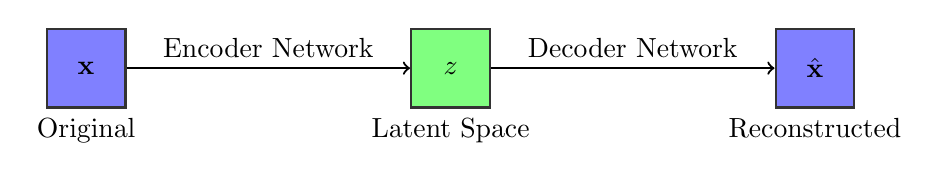
\begin{tikzpicture}
\tikzstyle{main}=[rectangle, minimum size = 10mm, thick, draw =black!80, node distance = 36mm]
\tikzstyle{connect}=[-latex, thick]
  \node[main, fill = blue!50] (alpha) [label=below: Original ] {$\x$};
  \node[main,fill = green!50] (z) [right=of alpha,label=below:Latent Space] { $z$};
  \node[main,fill = blue!50] (xout) [right= of z,label=below: Reconstructed ] {$\hat{\x}$ };
  \draw[thick,->] (alpha) -- (z) node[midway,sloped,above] {Encoder Network};
  \draw[thick,->] (z) -- (xout) node[midway,sloped,above] {Decoder Network};
  \end{tikzpicture}
\end{figure}

The loss function for a given input vector is usually the reconstruction error:
\[
\loss(\x) = \norm{ \x-\hat{\x}}^2
\]


\end{frame}

%%%%%%%%%%%%%%%%%%%%%%%%%%%%%%%%%%%%
\begin{frame}{Autoencoders}

  \begin{figure}[ht]
    \centering
    \includegraphics[width=0.5\textwidth]{ae.png}
  \end{figure}

  \begin{itemize}
  \item Encoder: $E$; decoder: $G$; autoencoder: $G \circ E$
  \item In most applications, the latent space is ``smaller'' than the data space.
  \item Objective: $\hat{x}$, i.e. $G \circ E (x)$, ``close'' to $x$
  \item When dealing with images, modern autoencoders use convolutional neural networks
  \end{itemize}

\end{frame}

%%%%%%%%%%%%%%%%%%%%%%%%%%%%%%%%%%%%
\begin{frame}{Generative adversarial networks \cite{goodfellow_generative_2014}}

  \begin{figure}[ht]
    \centering
    \includegraphics[width=0.5\textwidth]{gan2}
  \end{figure}

  \begin{itemize}
  \item The \alert{discriminator} $D$ is optimized so that it correctly classifies images as real (1) or fake (0)
  \item The decoder or \alert{generator} $G$ is optimized so that the produced images are classified as real by the discriminator
  \end{itemize}

  \begin{block}{Value function}
    $V(G,D) = \mathbb{E}_{p_\x}(log(D(\x))) + \mathbb{E}_{p_z(z)}(log(1 - D(G(z))))$
  \end{block}

\end{frame}

%%%%%%%%%%%%%%%%%%%%%%%%%%%%%%%%%%%%
\begin{frame}{Which face is real?}


\end{frame}


%%%%%%%%%%%%%%%%%%%%%%%%%%%%%%%%%%
\section{Conclusion}

%%%%%%%%%%%%%%%%%%%%%%%%%%%%%%%%%%%%
\begin{frame}{Conclusion}

\begin{itemize}
\item Deep learning allows to learn complex transformations between tensors, thanks to:
  \begin{itemize}
  \item Smart methods and algorithms
  \item Lots of data
  \item Specialized hardware
  \end{itemize}
  \item General artificial intelligence is still far away
\end{itemize}

\end{frame}




%%%%%%%%%%%%%%%%%%%%%%%%%%%%%%%%%%%%%%%%%%%%%%%%%%
\section*{References}

%%%%%%%%%%%%%%%%%%%%%%%%%%%%%%%%%%%%%%%%%%%%%%%%%%

\frame[allowframebreaks]{

  \scriptsize

  \frametitle{References}

  %\bibliographystyle{amsalpha}
  %\bibliographystyle{apalike}

  \bibliography{../../edf.bib,slides_deep.bib}

  \normalsize

}



\end{document}
